\documentclass[11pt]{article}
\usepackage[a4paper,margin=1in]{geometry}
\usepackage[T1]{fontenc}
\usepackage[utf8]{inputenc}
\usepackage{lmodern}
\usepackage{microtype}
\usepackage{amsmath,amssymb}
\usepackage{graphicx}
\usepackage{booktabs}
\usepackage{xcolor}
\usepackage{hyperref}
\usepackage[numbers,sort&compress]{natbib}
\usepackage{caption}
\usepackage{array}
\usepackage{url}
\hypersetup{colorlinks=true,linkcolor=blue!50!black,citecolor=blue!50!black,urlcolor=blue!50!black}
\hypersetup{pdftitle={Fine-Tuning a Language Model on Its Own Verified Lean Proofs: Transfer, Generalisation and Saturation Across Three Iterations},pdfauthor={Roberto I. Ono Filho}}
% Deposit placeholders: fill before depositing.
\newcommand{\reportdate}{5 October 2026}% date of this version
\newcommand{\thisdoi}{10.5281/zenodo.23163729}% DOI of this report
\newcommand{\evidencedoi}{10.5281/zenodo.23163299}% DOI of the deposited evidence archives
\captionsetup{font=small,labelfont=bf}
\graphicspath{{figures/}}
\setlength{\parskip}{0.25em}
\emergencystretch=1em
\renewcommand{\topfraction}{0.95}\renewcommand{\textfraction}{0.05}\renewcommand{\floatpagefraction}{0.8}
\newcolumntype{R}[1]{>{\raggedright\arraybackslash}p{#1}}

\title{Fine-Tuning a Language Model on Its Own Verified Lean Proofs:\\
Transfer, Generalisation and Saturation Across Three Iterations}
\author{Roberto I. Ono Filho\\ Independent researcher\\
\texttt{ono.roberto@gmail.com} \quad ORCID \href{https://orcid.org/0009-0006-8650-629X}{0009-0006-8650-629X}}
\date{\small Report, version 1, \reportdate. Frozen as draft 0.4 on 25 September 2026 after two rounds of review by AI reviewer agents; not peer reviewed and not submitted to a venue. Corrections after freezing are listed in Section~\ref{sec:corrections}. Zenodo: \href{https://doi.org/\thisdoi}{\thisdoi}.}

\begin{document}
\maketitle

\begin{abstract}
We ask whether a language model improves on problems it has not seen when
the proofs it produced and a verifier accepted are fine-tuned into its
weights, with no human selecting or editing them. The setting is a ladder
of six graded families of small Lean~4 worlds whose instances differ in
constants, not in structure. The loop ran for three iterations on a
served 27B model; every stage was read once against a pre-registered
rule, and every adapter was compared with one trained on the generator's
template proofs of the same cells. Template proofs write their form into
the weights: their adapter solves its trained steps at the first
submission and no others, and writes skeletons with guessed coefficients
that reasoning in context fills. The model's own accepted proofs transfer
within their steps and, at the second iteration, solve two steps for
which no template was shown; the loop stops at L4, whose invariant the
lineage produced twice in 48 sessions and the second adapter never writes
there. On four new families the loop's adapter rises over the base by the
rule in three, at a seventh to two fifths of the tokens, while the
template adapter of the same cells writes its nearest trained skeleton
and does not fall below the base. A third iteration raises how often the
needed kind of invariant is tried first and leaves the solve rate where
it was; a registered composition test did not fire. A hand-validated
classifier of the kind tried first (3,660 sessions) separates prior from
execution: consolidation moved the prior toward forms in the training
data; thinking and practice improved execution and repair; in three of
the four new families the loop's adapter guessed the needed kind less
often than the base and solved more by repairing after a rejection. Every
family an adapter solved, the base also solved at eight attempts and 131k
thinking tokens; at the level of instances and small budgets the adapters
cover more; support at larger budgets was not measured.
\end{abstract}

\section{The question}
\label{sec:question}

The previous papers of this series measured what an office-scale language
model does with a stimulus and with an idea it is handed
\citep{ono2026interrupting,ono2026mass,ono2026operator,ono2026pulsed}, and concluded that the model applies an idea it is handed in operable form but did not, in those programs, produce an operator of its own \citep{ono2026operable}. Weight consolidation appeared there once, in the
bin-packing lineages of the second paper, where it moved the mass of
proposals toward the known good and thinned the tails \citep{ono2026mass}.
This paper asks the question the series left open: when nothing is handed to the model and its only training data are its own verifier-accepted proofs, does it improve on instances it has not seen, and where does the improvement stop?

``Without selection'' means here that no human selects, edits, ranks or
orders the proofs that enter training; every accepted proof of a
production run enters as it came. The humans still supply the generator of
problems, its six graded steps, the verifier, the choice of which steps
each iteration attempts, and the decision to retrain from scratch on the
cumulative set. Automatic selection of training rationales is also how
STaR, ReST-EM and rejection-sampling fine-tuning work
\citep{zelikman2022star,singh2024restem,yuan2023scaling}, so the phrase describes the data regime only. The design's distinctive element is its matched control. A generator produces sibling
instances of a formal problem, a verifier decides, and for every instance
a template reference proof exists, so that each self-trained adapter can
be compared with an adapter trained on the reference proofs of exactly
the same cells. The program was run as eight pre-registered studies
(``nodes'') between 13 and 20 September 2026, each archived with a
SHA-256 manifest (Table~\ref{tab:nodes}; Figure~\ref{fig:design} shows
which arm was trained and read where). Each of the seven confirmatory
nodes was read once by a script written before its data (A8 also had a
declared second read, Section~\ref{sec:walls}); the descriptive node A6
registered its method and questions before it ran, and its scripts were
committed with its first read and rerun twice as later nodes added
sessions. The program's findings, stated without numbers here, with them
in the sections that follow, and summarised in Figure~\ref{fig:loop}:

\begin{enumerate}
\item \textbf{Template proofs write their form into the weights}
(Section~\ref{sec:curated}). An adapter trained on the reference proofs of
two steps solves those steps at the first submission and no others. The
six-form adapter solves the four steps whose measure is read off the moves
and fails the two whose parameters must be inferred, writing the right
skeleton with guessed coefficients. Reasoning in context fills the coefficients; the same change of sampling configuration without reasoning leaves the rate where it was.
\item \textbf{The loop closes without selection and climbs}
(Section~\ref{sec:loop}). The base's own accepted proofs, consolidated as
they came, transfer within their steps. The resulting adapter, thinking,
produces proofs of two higher steps for which no template was ever shown,
and their consolidation solves those steps at the first submission
without thinking. The loop stops at L4, the one step whose invariant, a
product of two different fields in a three-field world, the lineage
produced twice in 48 sessions and the adapter never writes there.
\item \textbf{On four new families the loop's adapter rises over the base
and the template adapter writes its nearest trained skeleton}
(Section~\ref{sec:walls}). The loop's adapter rises over the base in three
of the four families by the rule and in all four descriptively, at a
fraction of the tokens. The template adapter trained on the same cells
does not fall below the base, but writes in every first submission the
trained skeleton nearest to the world, and combines two skeletons far
less often than the loop.
\item \textbf{A third iteration saturates} (Section~\ref{sec:a9}). Adding
the adapter's own proofs of the new families raises how often the needed
kind of invariant is tried first and leaves the solve rate where it was;
it does not make the new families solvable without thinking; the
registered composition test did not fire.
\item \textbf{What is tried and what is executed can be separated}
(Section~\ref{sec:forms}). A classifier of the kind of invariant in the
first submission, validated by hand, shows that consolidation moved the
prior over forms and that thinking moved execution and repair. In three
of the four new families the loop's adapter guesses the needed kind at the
first submission less often than the base, and it solves more because it
repairs its guess after the verifier rejects it.
\end{enumerate}

\begin{figure}[!htbp]
\centering
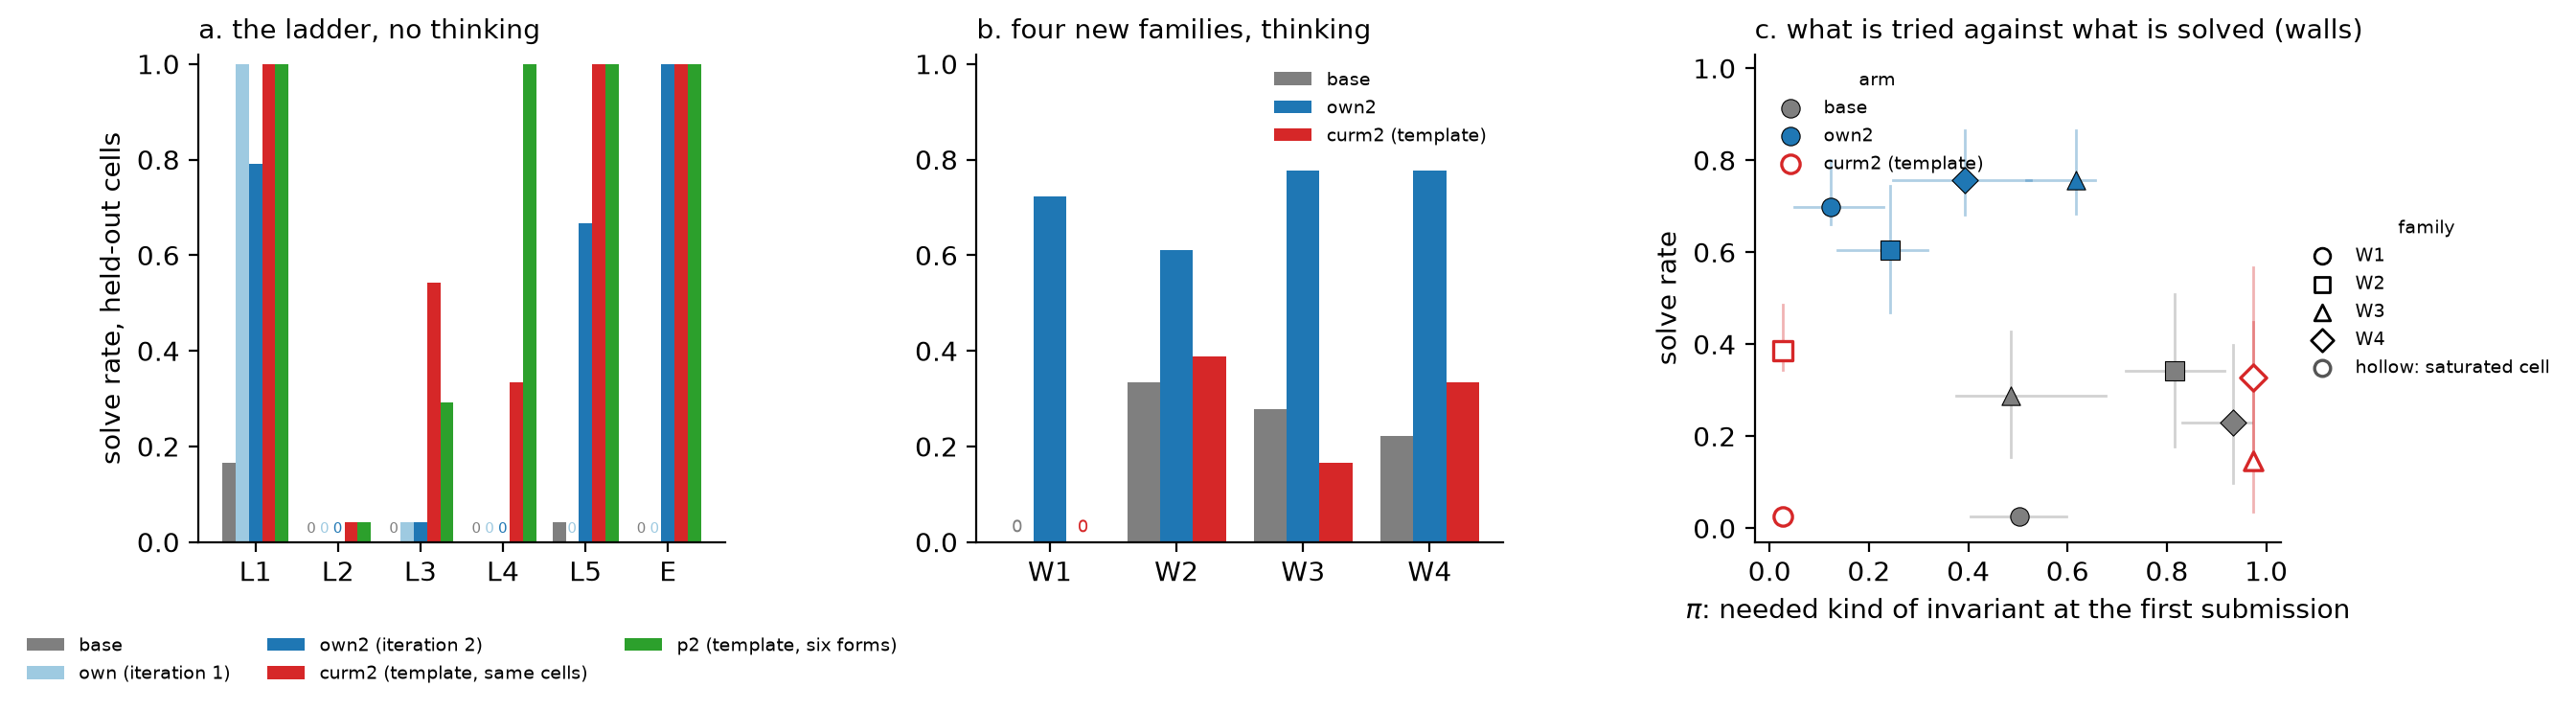
\includegraphics[width=\textwidth]{fig_loop.png}
\caption{The three results in one figure, from the read files; a zero-height bar is printed as 0. (a) Held-out solve rates on the ladder without thinking: the base, the two self-trained adapters (own, own2), the template adapter trained on own2's cells (curm2) and the six-form template adapter (p2). (b) The four new families with thinking: base, own2 and the template adapter of the same cells. (c) On the walls, what is tried against what is solved: $\pi$, the rate of the needed kind of invariant at the first submission (median and 90\% interval), against the solve rate, per arm and family; the lines are 90\% intervals, and a hollow marker is a saturated cell, where every session of every instance has or lacks the kind and $\pi$ sits at the smoothing floor or ceiling (Section~\ref{sec:forms}). The base and the template adapter tend to start with the needed kind and then fail to complete the proof; the loop's adapter tends to start with another kind and reach the needed one after a rejection.}
\label{fig:loop}
\end{figure}

\begin{table}[!htbp]
\centering\footnotesize
\setlength{\tabcolsep}{4pt}
\begin{tabular}{R{2.4cm} R{6.0cm} R{2.1cm} R{4.2cm}}
\toprule
node (read) & question and registered primary & sessions, GPU & registered verdict (plain English) \\
\midrule
A2 (14 Sept.) & does a template form write into the weights? primary: the form-specific adapter rises on its two steps and on no other & 576, US\$32 & \path{form_written_and_form_specific}: yes, and only that form \\
A2 replication, P4, E8 (14 Sept.) & new instances and adapters; does thinking complete the form? primary: same rises; the adapter with thinking rises over itself without thinking in the same configuration & 768, US\$75 & \path{replicated}; \path{reasoning_is_the_active_ingredient_given_the_form} \\
Loop, iteration 1 (15 Sept.) & do the model's own accepted proofs move it? primary: own rises over the base on its steps, without and with thinking & 528, US\$69 & \path{self_consolidation_moves}: yes \\
Loop, iteration 2 (16 Sept.) & does the ladder climb without selection? primary: own2 rises over the base at the two produced steps & 744, US\$112 & \path{ladder_climbs_without_curator}: yes, without thinking \\
A7 (17 Sept.) & is there a step the base never passes? wall: base 0 of 48 sessions at 131k tokens & 234, US\$91 & \path{not_a_wall_at_scale}: no candidate was a wall \\
A8, A8-c (19 Sept.) & does the template adapter narrow, does the loop's generalise? two-of-four-families rules & 216 (45 of them in the second read), US\$107 & \path{self_generalises_only} \\
A9 (20 Sept.) & does a third iteration compose (primary), cheapen, or saturate? & 594, US\$58 & \path{saturates} \\
A6 (19 Sept.) & what is tried versus what is executed & 3,660 (re-read) & secondary, descriptive \\
\bottomrule
\end{tabular}
\caption{The nodes. Sessions are distinct observed prover sessions; GPU cost is the rented H200 time of the node at list price, including the training of its adapters and its failures. The pre-registration commit of each node is listed in Appendix~\ref{app:ops}.}
\label{tab:nodes}
\end{table}

\section{Objects, arms and rules}
\label{sec:objects}

\paragraph{Terms.} An \emph{iteration} is one turn of the loop (produce,
consolidate, read). A \emph{session} is one attempt at one instance by one
arm; inside it the model makes up to twelve \emph{submissions}. An
\emph{attempt} count (``three attempts'') is the number of sessions per
instance and arm. A \emph{round} is one of the two rounds of the template
consolidation node. An \emph{arm} is a condition (weights and
configuration); a \emph{cell} is an instance, a step and an attempt. A
\emph{node} is one pre-registered study, and its \emph{read} is the single
execution of its registered analysis script on its complete data.

\begin{figure}[!htbp]
\centering
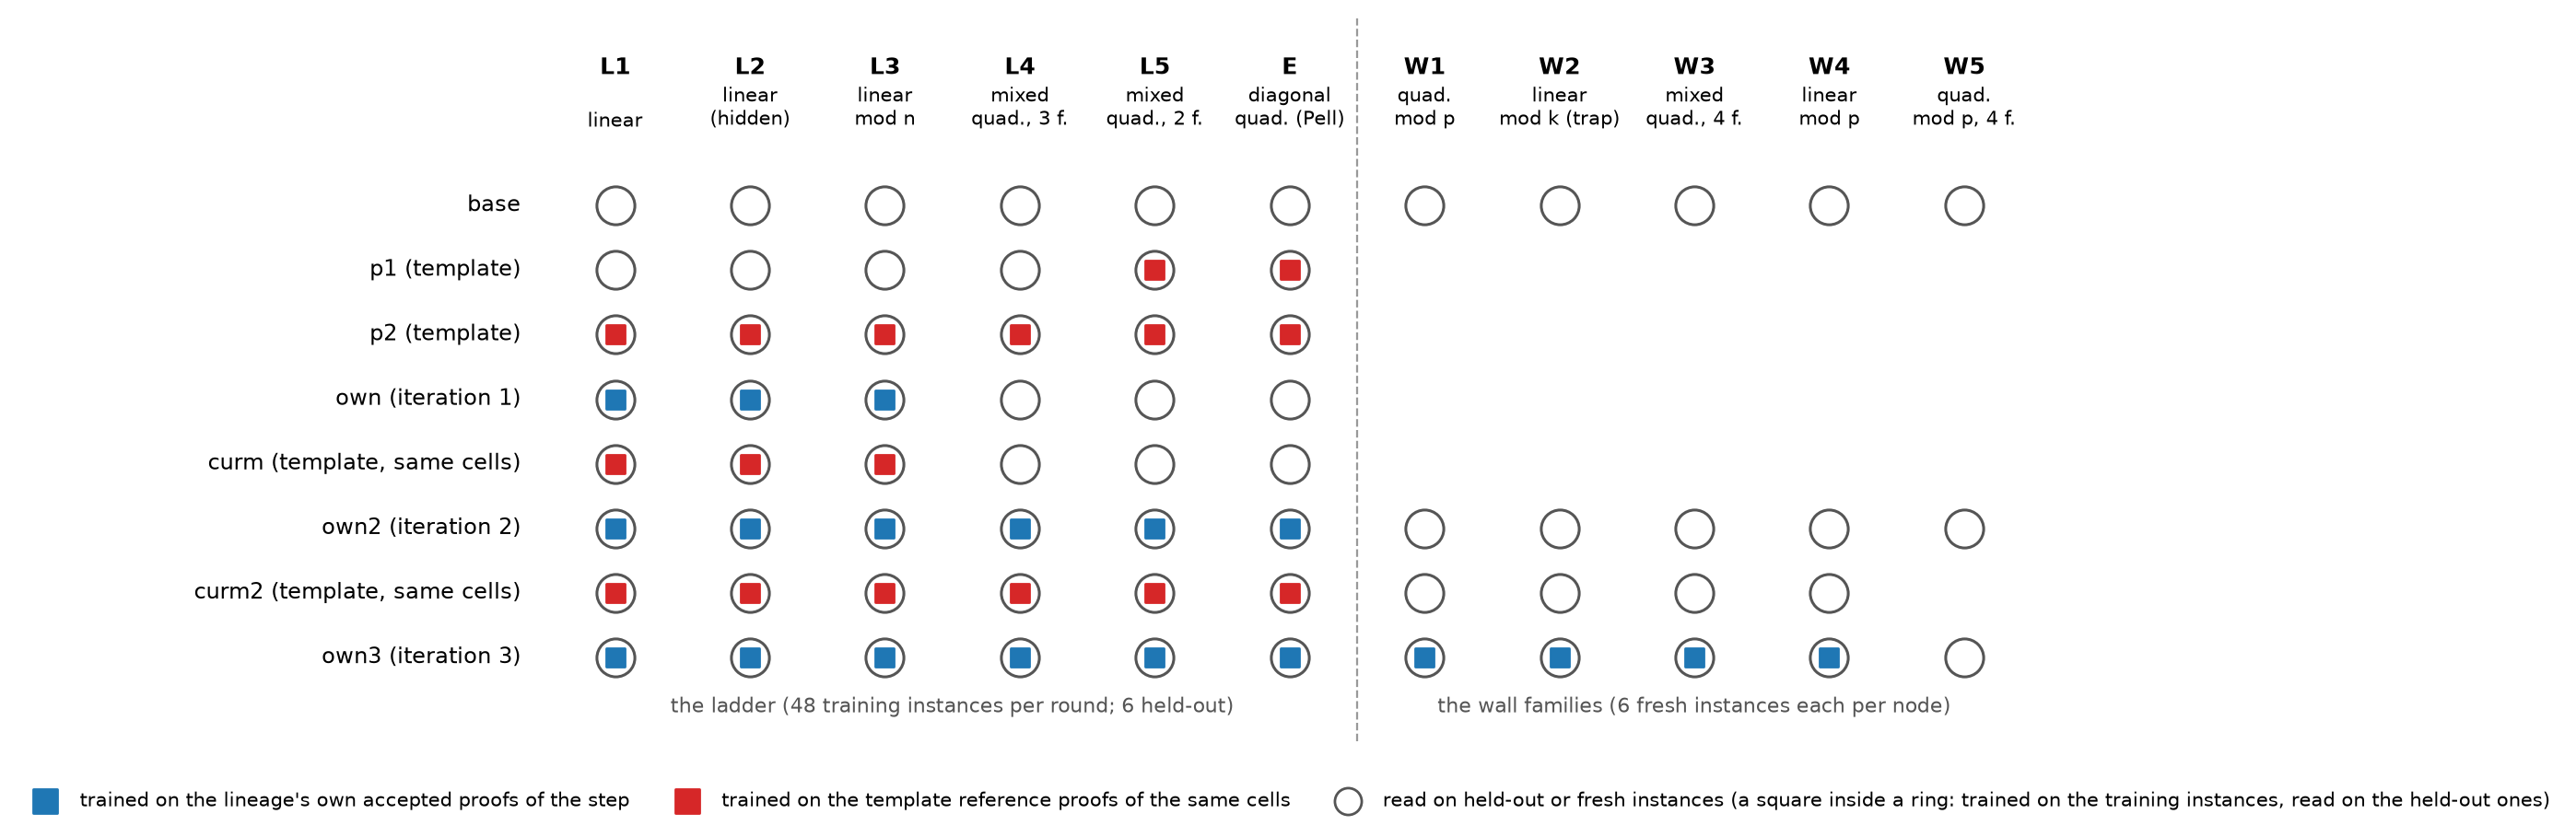
\includegraphics[width=\textwidth]{fig_design.png}
\caption{The design. Columns: the six ladder steps and the five wall families, each with the kind of invariant its intended proof needs (f.: fields of the state). Rows: the arms. A square marks what an adapter was trained on (blue: the lineage's own accepted proofs; red: the template reference proofs of the same cells); a ring marks where an arm was read, on held-out instances of the ladder or fresh instances of a family.}
\label{fig:design}
\end{figure}

\paragraph{The ladder.} A world is a small Lean~4 development
\citep{demoura2021lean4} over Mathlib \citep{mathlib2020}: a state of two
to four integer fields, four moves, a reachability relation, a start
state, and a target theorem stating that a family of states is
unreachable. The intended proof exhibits a quantity conserved by every
move (a \emph{measure}), proves conservation by induction on
reachability, and evaluates it on start and target. Six steps are graded
by the conserved quantity: L1, a difference of two fields; L2, a hidden
linear form $\alpha x+\beta y+z$; L3, a linear form modulo an index $n$;
L4, a quadratic form with offsets $(x-c_x)(z-c_z)-(y-c_y)^2$ under shears,
in three fields; L5, the form $x^2-kxy+y^2$ under the Vieta map, in two;
E, a Pell form $x^2-Dy^2$. Instances are seeded: they differ in their constants and share their structure, so ``held-out'' means held-out constants rather than
a shift of distribution. Every instance carries a reference proof accepted
by the same checker the sessions use and a mutation check (the reference
is rejected on a falsified world, and a witness proves the falsified
statement wrong). Six held-out instances drawn on 14 September for the
replication, and never trained on, serve every ladder reading after it
(the first round had its own six); 48 training instances per round serve
production and training.

\paragraph{The template proofs.} The reference proof of an instance is
emitted by the generator from one skeleton per step: a \texttt{measure}
definition, a step lemma, a bridge lemma by induction on reachability, and
a closing tactic (\texttt{omega} for the linear and modular steps,
\texttt{Int.sq\_nonneg} and \texttt{grind} for the quadratic ones). Across
the 288 reference proofs of a round there are six skeletons, one per step,
with the constants of each instance filled in. We call the adapters
trained on them \emph{template adapters}; the arm codes keep the
historical name \emph{curm} (``curated, matched''), and where the text
says ``curated'' it means these uniform reference proofs and nothing more
general.

\paragraph{The walls.} Four further families were built for the wall
search (Section~\ref{sec:walls}) in the same format: W1, a Pell form
conserved only modulo a prime $p$ under translations by $p$ (a composition
of E with L3); W2, a plane lattice whose exact linear invariant does not
separate start from target, so that a form modulo the lattice index is
needed (an L2 trap that requires L3); W3, a hyperbolic form in four fields
with offsets, preserved by SL$_2$ shears on two vectors; W4, the L3
construction with a prime between 11 and 19. A fifth, W5, was built for
the third iteration: the form of W3 conserved only modulo a prime, as in
W1. An exhaustive certificate checks, for every instance, that no exact
linear invariant separates start from target and no linear form modulo
$m\le30$ ($m\le12$ in four fields) does either, apart from the intended
family. Section~\ref{sec:a9} reports two shortcut families this
certificate did not cover, one of which also occurs in W1; the ladder had
no such certificate (Section~\ref{sec:corrections}).

\paragraph{The session.} A prover session shows the model the public files
of a world and asks for a complete Lean file proving the target
(Appendix~\ref{app:prompt} gives the prompt). Each submission is compiled
and checked (namespace, statement, standard axioms only); a rejection
returns the compiler's errors; the session ends at the first accepted
submission, at twelve submissions, at the output budget, or at the time
limit. Two configurations are used throughout: \emph{no thinking} (16,384
output tokens, $T$ 0.7, top-$p$ 0.8, 900\,s) and \emph{thinking} (131,072
tokens, $T$ 1.0, top-$p$ 0.95, 3,600\,s, the model's reasoning enabled).
Between submissions the conversation carries only the submitted file and
the errors; the reasoning of a rejected submission is not carried forward.
With thinking on, the model often writes the Lean file inside its
reasoning and leaves the answer empty; the file is then extracted from the
reasoning (an amendment recorded before the affected cells), so a ``first
submission'' under thinking is what the verifier received after the model
reasoned. An infrastructure failure (a dropped connection) is not an
observation, and the cell is rerun, at most three times.

\paragraph{Model and adapters.} The base is Qwen3.8-27B, a 2026 release of the Qwen3 line, served from the repository \texttt{Qwen/Qwen3.8-27B} of the Hugging Face Hub \citep{qwen2026qwen38}, downloaded afresh on each rented instance between 13 and 20 September 2026 (the repository revision was not recorded). It is the post-trained release rather than a pre-trained checkpoint: the two configurations above are its thinking and no-thinking modes, and the family's technical report \citep{qwen2025qwen3} describes the design in which the no-thinking mode is a distillate of the thinking mode. It is served in BF16 by vLLM 0.29.0 (transformers 5.17.0) on one
rented H200 (list price US\$4.59 per hour). Every adapter is a LoRA
\citep{hu2022lora} of rank 16 ($\alpha=32$, dropout 0.05) on the
attention and MLP projections, trained with peft 0.20.0 on torch 2.13
with AdamW at $2\times10^{-4}$, cosine schedule with 5\% warm-up,
effective batch 8, 4,096 tokens, bf16, for exactly 108 optimiser steps,
with the loss on the assistant tokens of a \texttt{[user: prover prompt,
assistant: proof]} pair rendered through the model's chat template with
thinking disabled. The last state is saved; there is no selection among
checkpoints; one training seed per adapter (2026091301 and 2026091402 for
the two rounds of A2; 2026091501, 2026091502 and 2026091901 for the three
iterations of the loop). Each iteration retrains from scratch on the
cumulative set. The same recipe and step count serve every adapter, so
that arms differ only in their data. Arm codes: \emph{base}; \emph{p1}
(96 reference proofs of E and L5), \emph{p2} (288 reference proofs of all
six steps), \emph{p3} (288 files with the same worlds, header and tactics
on a non-inductive target, a syntax control); \emph{own} (the 60 proofs
the base produced and the verifier accepted at L1--L3, iteration 1),
\emph{curm} (the reference proofs of exactly those 60 cells); \emph{own2}
(the 135 proofs of iterations 1 and 2, cumulative), \emph{curm2} (the
reference proofs of the same 135 cells); \emph{own3} (own2's data plus
the 52 proofs own2 produced on the wall families, iteration 3). A
trailing \emph{t} or the word \emph{thinking} marks the thinking
configuration.

\paragraph{The rule.} The unit of inference is the instance. For two arms
on the same cells, the paired difference of solve rates over the six
instances is tested by a one-sided sign-flip permutation ($p<0.05$; the
minimum with six instances is $0.0156$), once in each direction, and a
rise or fall is declared only if the pooled difference is also at least
$0.25$ in absolute value. Where a comparator sits above $0.75$ (ceiling)
or below $0.25$ (floor) the rule cannot fire, and this is reported rather
than worked around. The per-contrast level is not corrected for
multiplicity. The protection is that each node registered one primary
contrast or a conjunction of contrasts (``rises in at least two of four
families'') and a verdict vocabulary before any session ran, and was read
once by a script written before its data; every other contrast in the
tables is secondary and is marked as such in the captions. Descriptive
quantities (token counts, first-submission solves, the forms of the
submissions, the instance coverage) are reported as such. Amendments were
recorded with the clock time and before the cells they affected.

\section{Template proofs write the form}
\label{sec:curated}

Table~\ref{tab:curated} gives the two rounds. In both, the form-specific
adapter p1 solves E and L5 in 24/24 held-out cells, all at the first
submission, all with the trained skeleton, and moves nothing else. It
even loses the base's 4/24 at L1 by writing the Pell form $x\cdot x-y\cdot
y$ as a measure there (24/24 first submissions), a negative transfer
between forms. The six-form adapter p2 solves L1, L4, L5 and E in 24/24
and fails L2 (0 and 1 of 24) and L3 (7/24 in both rounds). In those two
steps it writes the right skeleton with guessed coefficients
($1\cdot x-2\cdot y+z$ where the world's form is, say, $-x-y+z$; $c$ and
$n$ guessed in $(x+c\,y)\bmod n$): it has learned the form of the proof but not how to derive the coefficients from the moves. The syntax
control p3 solves nothing in 288 sessions. The replication, with new
training instances, new held-out instances and adapters trained from
scratch, reproduces every cell to within one solve (base 5 and 5 of 144;
p1 48 and 48; p2 103 and 104; p3 0 and 0). Training losses fell to
$3.4\times10^{-3}$ or below, so the adapters memorised their examples, and the
transfer is to new constants rather than to the examples.
Section~\ref{sec:forms} qualifies ``only the form'': execution moved too
where the form has no parameter to infer, and at L3 it rose from 0.02 to
0.29, short of the ceiling.

\begin{table}[!htbp]
\centering\footnotesize
\begin{tabular}{lcccccc}
\toprule
arm & L1 & L2 & L3 & L4 & L5 & E \\
\midrule
\multicolumn{7}{l}{\emph{round 1 (13--14 September)}} \\
base, no thinking & 4/24 & 1/24 & 0/24 & 0/24 & 0/24 & 0/24 \\
p1: form of E/L5 (96 examples) & 0/24 & 0/24 & 0/24 & 0/24 & 24/24$\uparrow$ & 24/24$\uparrow$ \\
p2: six forms (288) & 24/24$\uparrow$ & 0/24 & 7/24 & 24/24$\uparrow$ & 24/24$\uparrow$ & 24/24$\uparrow$ \\
p3: syntax control (288) & 0/24 & 0/24 & 0/24 & 0/24 & 0/24 & 0/24 \\
\midrule
\multicolumn{7}{l}{\emph{replication, new instances and adapters (14 September)}} \\
base, no thinking & 4/24 & 0/24 & 0/24 & 0/24 & 1/24 & 0/24 \\
p1: form of E/L5 (96 examples) & 0/24 & 0/24 & 0/24 & 0/24 & 24/24$\uparrow$ & 24/24$\uparrow$ \\
p2: six forms (288) & 24/24$\uparrow$ & 1/24 & 7/24 & 24/24$\uparrow$ & 24/24$\uparrow$ & 24/24$\uparrow$ \\
p3: syntax control (288) & 0/24 & 0/24 & 0/24 & 0/24 & 0/24 & 0/24 \\
\bottomrule
\end{tabular}

\caption{Template consolidation, two rounds, six held-out instances $\times$ four attempts per step, no thinking. $\uparrow$: rise against the base by the rule. Registered primaries: p1 on E and L5; p2 on every step; p3 on none.}
\label{tab:curated}
\end{table}

\paragraph{Thinking fills the coefficients.} Table~\ref{tab:e8} isolates
what reasoning adds once the form is in the weights. With thinking on and
nothing else changed (same cells, same input hashes, the only differing
field of the agent being \texttt{enable\_thinking}), p2 goes from 2/24 to
19/24 at L2 and from 5/24 to 18/24 at L3 ($+0.71$ and $+0.54$,
$p=0.016$); the configuration alone (sampling temperature, budget, time)
moves nothing ($+0.04$, $-0.08$). In the sessions, the adapter writes the
skeleton with guessed coefficients, is rejected, and corrects the
coefficients in its second response with about 3,000 tokens; without
thinking it repeats the guess up to the twelve-submission limit against
the same error. The base with the same thinking reaches 6/24 and 8/24 at
about 100,000 tokens per session, never at the first submission, with
heterogeneous forms. So with the form in the weights, the remaining work,
deriving the coefficients, is done in context, and only when the model
can reason over the verifier's rejection.

\begin{table}[!htbp]
\centering\footnotesize
\begin{tabular}{llcccc}
\toprule
arm & weights & thinking & $T$ / top-$p$ & budget & L2 \quad L3 \\
\midrule
base & base & off & 0.7 / 0.8 & 16k & 0/24 \quad 0/24 \\
basen & base & off & 1.0 / 0.95 & 131k & 2/24 \quad 0/24 \\
baset & base & on & 1.0 / 0.95 & 131k & 6/24 \quad 8/24 \\
p2 & p2 & off & 0.7 / 0.8 & 16k & 1/24 \quad 7/24 \\
p2n & p2 & off & 1.0 / 0.95 & 131k & 2/24 \quad 5/24 \\
p2t & p2 & on & 1.0 / 0.95 & 131k & 19/24 \quad 18/24 \\
\midrule
\multicolumn{6}{l}{\emph{paired contrasts (rate difference, sign-flip $p$)}} \\
\multicolumn{5}{l}{p2t $-$ p2n (thinking, same configuration)} & +0.71 ($p=0.016$) \quad +0.54 ($p=0.016$) \\
\multicolumn{5}{l}{p2n $-$ p2 (configuration alone)} & +0.04 ($p=0.500$) \quad -0.08 ($p=0.938$) \\
\multicolumn{5}{l}{baset $-$ basen (thinking, no form)} & +0.17 ($p=0.125$) \quad +0.33 ($p=0.016$) \\
\multicolumn{5}{l}{p2t $-$ baset (form, both thinking)} & +0.54 ($p=0.016$) \quad +0.42 ($p=0.016$) \\
\bottomrule
\end{tabular}

\caption{The form and the reasoning, L2 and L3, six held-out instances $\times$ four attempts. The middle rows of each block share every cell and input with the thinking row; only \texttt{enable\_thinking} differs. Registered primary: p2t $-$ p2n; the others are secondary.}
\label{tab:e8}
\end{table}

\section{The loop without selection}
\label{sec:loop}

\paragraph{Iteration 1.} The base, thinking, tried once each of L1, L2 and
L3 on the 48 training instances and produced 60 accepted proofs (21, 23
and 16 of 48), none at the first submission, at a median of about 100,000
output tokens per session. The proofs are the model's own: with and
without auxiliary lemmas, induction closed by \texttt{omega},
\texttt{norm\_num}, \texttt{simp} or \texttt{linarith}. They were
consolidated as they came (no selection, no editing, no ordering) into
\emph{own}; the reference proofs of exactly those 60 cells gave
\emph{curm}. Table~\ref{tab:loop} (rows own, curm) and
Table~\ref{tab:contrasts} give the reading. Without thinking, own solves
L1 at 24/24 (base 4/24), 23 of them at the first submission, and 1/24 at
L2--L3 combined; with thinking it solves L2 at 21/24 and L3 at 19/24
against 6/24 and 8/24 for the base with the same thinking ($+0.62$ and
$+0.46$, $p=0.016$), and is within noise of the six-form template adapter
p2 with thinking (19/24, 18/24). Nothing moved at L4, L5 or E, where the
model had never produced proofs. The matched template control shows what the template adds: without thinking, curm solves L3 at the first
submission in 13/24 where own solves 1/24; with thinking, own reaches curm
spending roughly four to twenty times the tokens (medians 11,700 and
20,000 against 3,200 and 900), never at the first submission.

\paragraph{Iteration 2.} The adapter own, thinking, tried once each of L4,
L5 and E on the training instances and produced 75 accepted proofs: E
38/48, L5 35/48, L4 2/48. Consolidated cumulatively with the 60 of
iteration 1 (135 examples), it gives \emph{own2}; the 135 reference
counterparts give \emph{curm2}. Own2 solves E in 24/24 and L5 in 16/24
without thinking, at the first submission, at a median of about 540 tokens
per session, against 0/24 and 1/24 for the base without thinking and
12/24 and 10/24 for the base with 131k tokens of thinking ($+1.00$,
$p=0.016$; $+0.62$, $p=0.031$). This lineage was never shown a template of E or L5. The base produced proofs of L1--L3; own, trained on them, produced proofs of E and L5; own2, trained on those as well, solves E and L5 at the first submission. With thinking, own2 reaches 22/24 at both E and
L5 against 12 and 10 for the thinking base, with $p=0.062$ at both, five
instances up and one tied, below the registered threshold and reported as
such. Retention: no fall by the rule; descriptively, cumulative
consolidation lowered the rate at one lower step (L1, 24/24 to 19/24,
$-0.21$, $p=0.062$) and left the others unchanged (Table~\ref{tab:loop}).
One cell of that table has no explanation we can offer: the template
adapter of 135 cells (curm2) solves L3 without thinking in 13/24 where
the six-form template adapter of 288 proofs (p2) solves 7/24, with one
seed each.

\begin{table}[!htbp]
\centering\footnotesize
\begin{tabular}{lcccccc}
\toprule
arm & L1 & L2 & L3 & L4 & L5 & E \\
\midrule
\multicolumn{7}{l}{\emph{no thinking (16{,}384 tokens, $T$ 0.7)}} \\
base & 4/24 & 0/24 & 0/24 & 0/24 & 1/24 & 0/24 \\
own: 60 own proofs of L1--L3 (iteration 1) & 24/24 & 0/24 & 1/24 & 0/24 & 0/24 & 0/24 \\
curm: the reference proofs of the same 60 cells & 24/24 & 0/24 & 13/24 & 0/24 & 0/24 & 0/24 \\
own2: 135 own proofs, cumulative (iteration 2) & 19/24 & 0/24 & 1/24 & 0/24 & 16/24 & 24/24 \\
curm2: the reference proofs of the same 135 cells & 24/24 & 1/24 & 13/24 & 8/24 & 24/24 & 24/24 \\
p2: reference proofs of all six steps (288) & 24/24 & 1/24 & 7/24 & 24/24 & 24/24 & 24/24 \\
\midrule
\multicolumn{7}{l}{\emph{thinking (131{,}072 tokens, $T$ 1.0)}} \\
base & -- & 6/24 & 8/24 & 9/24 & 10/24 & 12/24 \\
own (iteration 1) & -- & 21/24 & 19/24 & -- & -- & -- \\
curm & -- & 17/24 & 18/24 & -- & -- & -- \\
own2 (iteration 2) & -- & 20/24 & 17/24 & 6/24 & 22/24 & 22/24 \\
curm2 & -- & 16/24 & 11/24 & 6/24 & 24/24 & 24/24 \\
p2 & -- & 19/24 & 18/24 & -- & -- & -- \\
\bottomrule
\end{tabular}

\caption{The loop, two iterations, six held-out instances $\times$ four attempts. Own and curm are trained on the same 60 cells; own2 and curm2 on the same 135; p2 on 288 reference proofs of all six steps. The thinking rows of iteration 1 were run at L2 and L3 only.}
\label{tab:loop}
\end{table}

\begin{table}[!htbp]
\centering\footnotesize
\begin{tabular}{lll}
\toprule
contrast & step & rate difference \\
\midrule
own $-$ base (no thinking) & L1 & +0.83 ($p=0.016$) \\
ownt $-$ baset & L2 & +0.62 ($p=0.016$) \\
ownt $-$ baset & L3 & +0.46 ($p=0.016$) \\
ownt $-$ p2t & L2 & +0.08 ($p=0.250$) \\
ownt $-$ p2t & L3 & +0.04 ($p=0.500$) \\
curm $-$ own (no thinking) & L3 & +0.50 ($p=0.062$) \\
\midrule
own2 $-$ base (no thinking) & L5 & +0.62 ($p=0.031$) \\
own2 $-$ base (no thinking) & E & +1.00 ($p=0.016$) \\
own2t $-$ baset & L4 & -0.12 ($p=0.844$) \\
own2t $-$ baset & L5 & +0.50 ($p=0.062$) \\
own2t $-$ baset & E & +0.42 ($p=0.062$) \\
curm2 $-$ own2 (no thinking) & L3 & +0.50 ($p=0.031$) \\
curm2 $-$ own2 (no thinking) & L4 & +0.33 ($p=0.250$) \\
\bottomrule
\end{tabular}

\caption{The contrasts of the two iterations (paired rate difference over six instances, one-sided sign-flip $p$). Registered primaries: iteration 1, own $-$ base (no thinking) and ownt $-$ baset; iteration 2, own2 $-$ base at L5 and E, own2t $-$ baset at L4, L5 and E; the rest are secondary.}
\label{tab:contrasts}
\end{table}

\paragraph{Where the loop stops: L4 and the mixed form.} L4 is where the
loop stops: production yielded two proofs in 48 sessions, and own2 solves
0/24 without thinking and 6/24 with it (base with thinking 9/24). Own2
declares a function of the state in 24 of 24 first L4 submissions, under
names such as \texttt{inv}, \texttt{q} or \texttt{state\_inv}, but of the
wrong kind: a linear form in 16 and a diagonal quadratic form
($x^2-2y^2+z^2$ with offsets) in 8. The mixed term that L4 requires, a
product of two different fields such as $(x-4)(z-3)$, appears in 0 of 24,
and in no submission of any session. The template adapters write the
mixed term in 20 of 20 and 21 of 21 first submissions; the thinking base
in 14 of 22 (13 by the classifier of Section~\ref{sec:forms}); own2 with thinking in 1 of 24 first submissions and in 11 of
24 sessions at some point (6 solved). Two further facts bear on this. First, the
two own L4 proofs that did enter own2's data were of the mixed form, and
so were the two reference proofs of the same cells in curm2's data; the two template examples suffice for curm2 to write the mixed form in every first submission, while the two own examples leave own2's first submissions unchanged. In the template set
the L4 form is one more instance of a skeleton the adapter learned from
all 135 examples; in the self-produced set it is two proofs among 135
heterogeneous ones. Second, the prior is conditional on the world's
shape. By the taxonomy of Section~\ref{sec:forms} the L5 form
$x^2-kxy+y^2$ is also a mixed quadratic, own2's data hold 28 such proofs
from L5, and own2 writes that kind in 24 of 24 first submissions at L5 and
in 0 of 24 at L4: it produced the mixed form in the two-field worlds of
the Vieta map and did not carry it to the three-field worlds of L4 with
shear moves, where its own two productions were too few. (A first reading
of this node counted the name \texttt{measure}, the name of our reference
proofs, and concluded that the loop's adapters ``never declare a
measure''; the count above, of what is written, replaced it on 19
September, and the classifier of Section~\ref{sec:forms} reproduces it:
16 linear, 8 diagonal, 0 mixed.)

\section{Out of the training distribution}
\label{sec:walls}

\paragraph{The wall search: no candidate met the definition.} To ask whether the loop
passes a step the base never passes, four candidate families were built
(W1--W4, Section~\ref{sec:objects}) and screened with three arms, eight
sessions each: the base thinking; the base thinking with the complete
reference proof of a \emph{sibling} instance of the same family shown as a
worked example; and own2 (Table~\ref{tab:walls}). Three candidates fell at
the screen. W1 (base 0/8) went to a confirmation on six new instances with
eight attempts each: the base solved 6/48, on four of the six instances,
and own2 30/48, on all six. The registered definition of a wall is a
support statement at one budget (base 0 of 48 sessions at 131k tokens),
not a statement of difficulty, so one solve is enough, and the 0/8 of the
screen was compatible with a rate of about ten per cent. Own2's rise
($+0.50$, $p=0.016$) is recorded, but the registered crossing rule applies
only to a confirmed wall. In 33 of 48 base sessions the model writes, at
some submission, the quadratic form modulo $p$ that the family needs, and
in 45 some modular invariant (by the classifier of
Section~\ref{sec:forms}; the coarser count of sessions attempting anything
modular, made at the time of the node, was 29): it has the right idea, and
then fails to complete the Lean proof, ending at the 131k-token ceiling;
the sibling proof unlocks it (19/24). A worked proof supplies the idea and the form together, so this test cannot tell which of the two the base was missing.

\begin{table}[!htbp]
\centering\footnotesize
\begin{tabular}{lcccl}
\toprule
candidate & base & base + sibling proof & own2 & class \\
\midrule
W1 Pell form modulo a prime & 0/8 & 6/8 & 7/8 & wall\_candidate \\
W2 plane lattice (trap) & 4/8 & 7/8 & 3/8 & not\_a\_wall \\
W3 hyperbolic form, four fields & 2/8 & 8/8 & 7/8 & not\_a\_wall \\
W4 large prime & 3/8 & 7/8 & 7/8 & not\_a\_wall \\
\midrule
\multicolumn{5}{l}{\emph{confirmation of W1, six new instances}} \\
W1 & 6/48 & 19/24 & 30/48 & not\_a\_wall\_at\_scale \\
\multicolumn{5}{l}{curm2, the template adapter (descriptive, cut by the guard): 0/18; own2 $-$ base +0.50 ($p=0.016$)} \\
\bottomrule
\end{tabular}

\caption{The wall search: screen (eight sessions per candidate and arm) and the confirmation of the one candidate (six new instances; base and own2 $\times 8$, base with the sibling proof $\times 4$, template adapter $\times 4$, cut short at 18 sessions by the automatic removal deadline of the rented instance). Secondary contrasts only: the registered rule was the wall definition.}
\label{tab:walls}
\end{table}

\paragraph{Generalisation against the template, on the same cells.} The
confirmation left a side finding: on W1 the template adapter curm2,
trained on the same 135 cells as own2, solved 0/18 and never tried
anything modular, while own2 solved 30/48. Node A8 then measured it: base, own2 and curm2, thinking, on six fresh instances of each of the four
families, three attempts each, with two rules registered before the data
(\emph{narrowing}: curm2 falls against the base in at least two of four
families; \emph{generalisation}: own2 rises against the base in at least
two). The node's read, made with the template arm at 27 of 72 cells after
three operational failures to complete it, gave
\texttt{self\_generalises\_only}; a second read, declared as such before
any new cell and made with the arm complete, gave the same verdict
(Table~\ref{tab:a8}). Own2 rises against the base in W1, W3 and W4 by the
rule (52/72 in all, against 15/72; W2 $+0.28$, $p=0.125$), at a seventh
to two fifths of the tokens by family (medians of 19,000 to 52,000
against 100,000 to 131,000). Curm2 does not narrow below the base: 16/72
against 15/72, with no family falling by the rule. Its deficit is against the loop's adapter: by the rule in W1 and W3; in W2 ($+0.22$, $p=0.062$) and W4 ($+0.44$, $p=0.078$) short of the rule on $p$.
Table~\ref{tab:coverage} gives the same data as instance coverage: at
three attempts the base solves at least one session on 0, 4, 4 and 3 of
the six instances of W1--W4, the template adapter on 0, 6, 1 and 4, and
own2 on all six of every family.

\begin{table}[!htbp]
\centering\footnotesize
\setlength{\tabcolsep}{3pt}
\resizebox{\textwidth}{!}{\begin{tabular}{lcccccc}
\toprule
family & base & own2 & curm2 (template) & own2 $-$ base & curm2 $-$ base & own2 $-$ curm2 \\
\midrule
W1 & 0/18 & 13/18 & 0/18 (node read 0/4) & +0.72 ($p=0.016$)$\uparrow$ & +0.00 ($p=1.000$) & +0.72 ($p=0.016$)$\uparrow$ \\
W2 & 6/18 & 11/18 & 7/18 (node read 1/6) & +0.28 ($p=0.125$) & +0.06 ($p=0.500$) & +0.22 ($p=0.062$) \\
W3 & 5/18 & 14/18 & 3/18 (node read 1/9) & +0.50 ($p=0.031$)$\uparrow$ & -0.11 ($p=0.375$) & +0.61 ($p=0.031$)$\uparrow$ \\
W4 & 4/18 & 14/18 & 6/18 (node read 3/8) & +0.56 ($p=0.031$)$\uparrow$ & +0.11 ($p=0.375$) & +0.44 ($p=0.078$) \\
\bottomrule
\end{tabular}
}
\caption{Generalisation against the template, four new families, six fresh instances each, three attempts, thinking. The template column is the complete arm of the second read, with the node read's partial count in parentheses; base and own2 are the same in both reads. Registered rules: own2 $-$ base rises in at least two families; curm2 $-$ base falls in at least two. own2 $-$ curm2 is secondary.}
\label{tab:a8}
\end{table}

\begin{table}[!htbp]
\centering\footnotesize
\resizebox{\textwidth}{!}{\begin{tabular}{llll}
\toprule
block & arm & attempts per instance & instances with at least one solve \\
\midrule
W1 (A7 confirmation) & base & 8 & W1 4/6 \\
W1 (A7 confirmation) & own2 & 8 & W1 6/6 \\
W1 (A7 confirmation) & base + sibling proof & 4 & W1 6/6 \\
W1 (A7 confirmation) & curm2, template (cut short) & 2--4 & W1 0/6 \\
\midrule
W1--W4 (A8) & base & 3 & W1 0/6, W2 4/6, W3 4/6, W4 3/6 \\
W1--W4 (A8) & own2 & 3 & W1 6/6, W2 6/6, W3 6/6, W4 6/6 \\
W1--W4 (A8) & curm2 & 3 & W1 0/6, W2 6/6, W3 1/6, W4 4/6 \\
\midrule
W1--W4, fresh instances (A9) & own2 & 3 & W1 6/6, W2 6/6, W3 6/6, W4 6/6 \\
W1--W4, fresh instances (A9) & own3 & 3 & W1 4/6, W2 6/6, W3 6/6, W4 6/6 \\
\midrule
W5 (A9) & base & 3 & W5 1/6 \\
W5 (A9) & own2 & 3 & W5 4/6 \\
W5 (A9) & own3 & 3 & W5 6/6 \\
\midrule
ladder, thinking (iteration 2) & base & 4 & L4 6/6, L5 6/6, E 5/6 \\
ladder, thinking (iteration 2) & own2 & 4 & L4 3/6, L5 6/6, E 6/6 \\
ladder, thinking (iteration 2) & curm2 & 4 & L4 2/6, L5 6/6, E 6/6 \\
\bottomrule
\end{tabular}
}
\caption{Support at small budgets: instances with at least one accepted proof, at the attempts each block ran (descriptive). No block measured more than eight attempts per instance.}
\label{tab:coverage}
\end{table}

The template adapter's first submissions are uniform within each family.
They are the same kind of invariant in 18 of 18 sessions: the exact Pell
form in W1 (never the modulus; 0/18 solved), the exact linear form in W2
(the trap; 8 sessions later repair it to a modulus and 7 solve), the
bilinear form with offsets in W3 (the right kind; 3/18 solved), and the
L3 measure $(\ldots)\bmod p$ in W4 (the right kind; 6/18). Where the
obstruction is the combination of two trained skeletons (a quadratic form
and a modulus in W1; a linear form and a modulus in W2), it attempts the
combination in 8 of 36 sessions, the base in 35 of 36 and the loop's
adapter in 36 of 36; it never adds a modulus to a quadratic form. The two
adapters differ in how often they combine skeletons and in which
combinations they attempt: the template adapter writes its nearest
trained skeleton and repairs only by appending a modulus to a linear form;
the loop's adapter starts from a wider set of forms and combines them
(repair rates in Section~\ref{sec:forms}).

\section{The third iteration saturates}
\label{sec:a9}

The loop was turned once more with what it had just produced: the 52
proofs own2 wrote on the wall families were added to its data (187
examples; the 24 instances of A8 became training instances) and
consolidated into \emph{own3}. Three questions were registered: does own3
\emph{compose} (the primary: rise against own2, thinking, on W5, a new
family that needs the form of W3 conserved only modulo a prime as in W1);
does it \emph{cheapen} (rise against own2 without thinking on at least two
of W1--W4, on 24 fresh instances); does it \emph{retain} (no fall against
own2 on the six ladder steps without thinking, nor on W1--W4 with
thinking). Table~\ref{tab:a9} gives the read: \texttt{saturates}. On W5
own3 solves 9/18 against 7/18 for own2 ($+0.11$, $p=0.375$), with six
instances and own2 already at 0.39, a test of little power. Without
thinking, nothing moves on the new families (3/72 against 0/72, every
family on the floor). There is no fall by the rule anywhere
(descriptively, E 24/24 $\to$ 21/24). A plateau after two or three
iterations is what the self-training literature reports
\citep{singh2024restem,zelikman2022star}, and this result replicates it on
a new substrate; what did change at the third iteration is described next.

\begin{table}[!htbp]
\centering\footnotesize
\setlength{\tabcolsep}{3pt}
\resizebox{\textwidth}{!}{\begin{tabular}{lccccl}
\toprule
block & own3 & own2 & base & own3 $-$ own2 & note \\
\midrule
W5, thinking (primary) & 9/18 & 7/18 & 1/18 & +0.11 ($p=0.375$) & own3 $-$ base +0.44 ($p=0.016$)$\uparrow$ \\
W5, no thinking & 0/18 & 0/18 & -- & +0.00 ($p=1.000$) & \\
W1 new instances, no thinking & 2/18 & 0/18 & 0/18 & +0.11 ($p=0.250$) & \\
W2 new instances, no thinking & 1/18 & 0/18 & 0/18 & +0.06 ($p=0.500$) & \\
W3 new instances, no thinking & 0/18 & 0/18 & 0/18 & +0.00 ($p=1.000$) & \\
W4 new instances, no thinking & 0/18 & 0/18 & 2/18 & +0.00 ($p=1.000$) & \\
W1 new instances, thinking & 8/18 & 9/18 & -- & -0.06 ($p=0.500$) & \\
W2 new instances, thinking & 15/18 & 13/18 & -- & +0.11 ($p=0.312$) & \\
W3 new instances, thinking & 14/18 & 11/18 & -- & +0.17 ($p=0.250$) & \\
W4 new instances, thinking & 12/18 & 14/18 & -- & -0.11 ($p=0.391$) & \\
ladder L1, retention, no thinking & 20/24 & 19/24 (16 Sept.) & -- & +0.04 ($p=0.500$) & \\
ladder L2, retention, no thinking & 2/24 & 0/24 (16 Sept.) & -- & +0.08 ($p=0.500$) & \\
ladder L3, retention, no thinking & 2/24 & 1/24 (16 Sept.) & -- & +0.04 ($p=0.500$) & \\
ladder L4, retention, no thinking & 2/24 & 0/24 (16 Sept.) & -- & +0.08 ($p=0.500$) & \\
ladder L5, retention, no thinking & 17/24 & 16/24 (16 Sept.) & -- & +0.04 ($p=0.500$) & \\
ladder E, retention, no thinking & 21/24 & 24/24 (16 Sept.) & -- & -0.12 ($p=0.250$) & \\
\midrule
\multicolumn{6}{l}{W5 solved by the intended route (quadratic form modulo $p$), post hoc: base 1/18, own2 4/18, own3 8/18} \\
\bottomrule
\end{tabular}
}
\caption{The third iteration, all blocks complete (594 sessions, none lost). Own3 and own2 are compared on identical cells; the ladder comparator is own2's run of 16 September on the same cells. Registered primary: own3 $-$ own2 on W5 with thinking; own3 $-$ base on W5 is secondary.}
\label{tab:a9}
\end{table}

Four descriptive observations accompany the verdict. First, the loop's
adapters solve a family the base barely does: W5 is hard for the base
(1/18, one instance, 13 sessions at the token ceiling); own3 and own2 solve
9/18 and 7/18 on six and four instances, and own3 against the base is
$+0.44$ ($p=0.016$), a secondary contrast. Second, the third iteration
raised the rate of the needed kind at the first submission without
raising the solve rate. Thinking, own3 writes the needed kind of invariant
at the first submission in 13/18, 9/18 and 17/18 sessions of W1--W3
against 4/18, 0/18 and 5/18 for own2, and the totals solved are 49/72 and
47/72; own3 writes at the first submission the kind own2 reached only after a rejection (at W3 this cuts
the tokens to a quarter, medians 17,000 against 61,000). Without thinking, the first submission moves in the same way but the proof is not completed: own3 writes the needed
kind in 14/18 (W1) and 18/18 (W3) first submissions and solves 2 and 0.
Third, without thinking the loop's adapter behaves like the template one.
On W5 it writes the skeleton of W3, the exact bilinear form, in 18 of 18
first submissions and never the composition; with thinking, the same
weights attempt the composition in 14 of 18 sessions (own2 in 7, the base
in 12). In these sessions the combination of two forms appeared only in
the thinking configuration (14 of 18 sessions against 0 of 18 without
thinking), while each individual form appeared in both. Fourth, the same movement reaches the ladder: on the held-out L4 instances without thinking, own3 writes the mixed kind in 21 of 24 first submissions, where own2 wrote it in 0 of 24, and in 13 of the 24 the function it declares is the world's reference measure exactly, offsets included (post hoc, 25 September, by polynomial comparison with the hidden reference measure); it solves 2 of 24 (own2 0 of 24), both among those 13, and the other eleven sessions with the exact measure end without an accepted proof. The 52 proofs added at the third iteration include the 14 W3 proofs, whose invariant is a mixed quadratic form in four fields with offsets; the kind carried to the three-field worlds of L4, and the execution did not follow.

\paragraph{A defect of the instrument.} Reading the accepted W5 proofs
exposed two shortcut families the certificate did not test: order
invariants (W5 has no inverse moves, so a region such as $x\ge a\wedge y\ge b$
can be closed under the moves with the target outside it) and the modular
orbit of a pair of linear forms $(x+z,\,y+w)$. Four of the seventeen
accepted W5 proofs used one of them (own2 three, own3 one); by the
intended route the counts are base 1, own2 4, own3 8 of 18, and the
post-hoc contrast own3 $-$ own2 is $+0.22$ ($p=0.11$), which would not have
passed the rule either. The second family also occurs in W1: 13 of its
100 accepted proofs close a set of residues of $(x,y)$ modulo $p$ without
the quadratic form, including three of the base's six in the A7
confirmation (by the intended route 3 of 48, on two of six instances), six
of own2's 37 in A7, two of the sibling arm's 19, one of own2's 13 in A8
and one of own3's 8 in A9. No verdict changes: the verifier accepted these
proofs, so they count under the registered rule, and the reads stand as
registered. No W5 proof entered a training set, since own3 was trained
before A9; own3's data do contain shortcut proofs of other families (one
W1 proof from A8 and seventeen ladder proofs at L2, E and L5 by an invariant
of another kind than the intended one, Section~\ref{sec:corrections}), a
risk that consolidation without selection carries by construction
\citep{setlur2024incorrect}. A further family would have needed inverse
moves, or a certificate testing order invariants and residue sets of
pairs; none was built, as the line of work closed on 25 September 2026.

\section{What is tried, and what is executed}
\label{sec:forms}

Several of the results above turned on the first submission. Node A6 measured it directly: for every observed prover session of the base and its
adapters (3,660 sessions in 42 conditions), a heuristic classifier over
the Lean source the verifier received labels the kind of invariant the
first submission declares (\emph{linear}, \emph{linear modulo},
\emph{diagonal quadratic}, \emph{mixed quadratic}, \emph{quadratic modulo},
\emph{none}; Appendix~\ref{app:forms}). The classifier was validated by
labelling sessions by reading before seeing its label: 57 of 60 in a
first stratified sample; after closing the two gaps that sample exposed
(the \texttt{ZMOD} notation; invariance stated as a relation between two
states), 40 of 40 in a second, fresh sample, and 99 of the 100 overall
with the corrected version. Each step has a needed kind fixed by its
generator. For a condition and a step, $\pi$ is the rate of the needed
kind at the first submission, $\theta_{\text{right}}$ the solve rate of the
sessions that started with it, $\theta_{\text{wrong}}$ that of the others;
intervals are a Bayesian bootstrap over instances (Dirichlet weights,
4,000 replicates, Jeffreys smoothing), paired when two conditions share
their instances. Two cautions apply to these quantities. Conditioning on the first kind
conditions on a post-treatment variable, so $\theta$ is a descriptive quantity and cannot be read as a causal effect. And where every session of every instance
has the kind, the smoothing floor prints as 0.98 or 0.02 with a degenerate
interval, and a contrast between two such cells clamps at about seven
nats; the tables print those cells as saturated rather than as estimates.
Table~\ref{tab:a6c} gives the contrasts and Appendix~\ref{app:pitheta}
the values per condition.

\begin{table}[!htbp]
\centering\footnotesize
\setlength{\tabcolsep}{4pt}
\resizebox{\textwidth}{!}{\begin{tabular}{llccc}
\toprule
contrast & step & $\Delta\,\mathrm{logit}\,\pi$ & $\Delta\,\mathrm{logit}\,\theta_{\text{right}}$ & $\Delta\,\mathrm{logit}$ rate \\
\midrule
p2 $-$ base, no thinking (replication) & L1 & 0 (sat.) & +5.37 [+5.04, +6.08] & +5.37 [+5.04, +6.08] \\
p2 $-$ base, no thinking (replication) & L2 & +3.52 [+2.73, +4.50] & +0.43 [-0.62, +1.53] & +0.96 [+0.12, +1.95] \\
p2 $-$ base, no thinking (replication) & L3 & +1.49 [+0.23, +2.75] & +2.92 [+1.95, +3.74] & +3.00 [+2.14, +3.77] \\
p2 $-$ base, no thinking (replication) & L4 & $>$+7 (sat.) & -- & $>$+7 (sat.) \\
p2 $-$ base, no thinking (replication) & L5 & +4.78 [+4.43, +4.93] & +5.53 [+4.15, +6.50] & +6.79 [+5.79, +7.67] \\
p2 $-$ base, no thinking (replication) & E & +5.16 [+4.63, +5.90] & +6.29 [+5.67, +6.67] & $>$+7 (sat.) \\
\midrule
own2 $-$ base, walls, thinking & W1 & -1.91 [-2.79, -1.46] & -- & +4.46 [+4.28, +5.03] \\
own2 $-$ base, walls, thinking & W2 & -2.69 [-3.75, -1.93] & +1.89 [+0.99, +3.01] & +1.09 [+0.40, +2.03] \\
own2 $-$ base, walls, thinking & W3 & +0.54 [-0.62, +1.13] & +2.31 [+0.56, +4.06] & +2.10 [+1.17, +3.27] \\
own2 $-$ base, walls, thinking & W4 & -3.03 [-4.15, -1.99] & +1.96 [+0.78, +3.36] & +2.42 [+1.37, +3.56] \\
\midrule
curm2 $-$ base, walls, thinking & W1 & -3.62 [-4.01, -3.21] & -- & 0 (sat.) \\
curm2 $-$ base, walls, thinking & W2 & -5.10 [-5.98, -4.55] & -- & +0.23 [-0.38, +0.97] \\
curm2 $-$ base, walls, thinking & W3 & +3.66 [+2.86, +4.11] & -1.46 [-3.08, -0.25] & -0.81 [-2.45, +0.65] \\
curm2 $-$ base, walls, thinking & W4 & +0.98 [+0.13, +2.03] & +0.50 [-0.66, +1.55] & +0.57 [-0.57, +1.61] \\
\midrule
own2 $-$ curm2, walls, thinking & W1 & +1.68 [+0.69, +2.44] & -- & +4.46 [+4.28, +4.98] \\
own2 $-$ curm2, walls, thinking & W2 & +2.48 [+1.77, +2.84] & -- & +0.88 [+0.45, +1.24] \\
own2 $-$ curm2, walls, thinking & W3 & -3.12 [-3.54, -2.97] & +3.78 [+2.25, +5.53] & +2.94 [+1.18, +4.73] \\
own2 $-$ curm2, walls, thinking & W4 & -4.03 [-4.67, -3.50] & +1.53 [-0.12, +3.42] & +1.84 [+0.62, +3.45] \\
\midrule
own2 $-$ curm2, L4, no thinking & L4 & -5.68 [-7.36, -4.11] & -- & -3.15 [-4.51, -1.59] \\
\midrule
own2 $-$ base, L4, thinking & L4 & -3.13 [-4.19, -1.68] & -- & -0.55 [-1.92, +0.44] \\
\midrule
p2t $-$ p2n (thinking given the form) & L2 & -0.96 [-1.97, -0.11] & +3.72 [+2.75, +5.07] & +3.52 [+2.66, +4.67] \\
p2t $-$ p2n (thinking given the form) & L3 & -1.66 [-2.38, -0.69] & +2.72 [+2.26, +3.30] & +2.37 [+1.81, +3.04] \\
\midrule
baset $-$ basen (thinking without the form) & L2 & +1.03 [+0.55, +1.57] & +1.55 [+0.42, +2.60] & +1.25 [+0.39, +2.52] \\
baset $-$ basen (thinking without the form) & L3 & -0.85 [-1.69, +0.05] & +3.09 [+2.61, +3.62] & +3.21 [+2.94, +3.58] \\
\bottomrule
\end{tabular}
}
\caption{Contrasts in nats (difference of logits), median and 90\% interval of the Bayesian bootstrap; rows share their instances and are paired. ``sat.'': both cells at the smoothing floor or ceiling, a clamp rather than a measured difference. Descriptive; no rule.}
\label{tab:a6c}
\end{table}

Four readings, each registered as a question with a prediction before the
tables were run. (Q1) Template consolidation moves $\pi$ to the ceiling
at every step and moves $\theta$ only where the form has no parameters to
infer: at L2 $\theta$ does not move; at L3 it rose 2.9 nats, against the
prediction, to 0.29, still far from one. (Q2) In three of the four wall
families the loop's adapter has a lower $\pi$ than the base at the first
submission (0.12, 0.24 and 0.39 at W1, W2 and W4 against 0.50, 0.82 and
0.93; at W3, 0.62 against 0.49). It starts with the simplest form of its
repertoire, is rejected, and repairs: of the sessions that start with the
wrong kind, 10 of 16 in W1, 14 of 14 in W2 and 9 of 11 in W4 reach the
needed one, and 24 of them solve. The base almost never repairs (0 of 9 in
W1) and, when it starts with the needed kind, rarely completes the proof
(W1 0/9, W2 4/15, W4 4/17). The template adapter has $\pi$ at the ceiling
where a trained skeleton serves and at the floor where two must be
combined, repairs only in W2 (8 of 18 sessions, 7 solved) and executes the
needed kind poorly ($\theta_{\text{right}}$ 0.15 at W3 against 0.89 for
the loop). Out of distribution, the loop's adapter improved in execution
and in repair after a rejection rather than in its initial guess. (Q3) At L4 the second iteration's adapter fails at the first guess: $\pi$ is 0.02 without thinking and 0.05 with it, against 0.85 for the template adapter and 0.54 for the thinking base; of the 23 thinking sessions that start with another kind, 10 reach
the mixed one later and 5 of those solve, and the 13 that never reach it solve none. After the third iteration, with fourteen four-field mixed proofs of W3 in the data, $\pi$ at L4 without thinking is 0.86 (in 13 of 24 sessions the exact reference measure, counted post hoc on 25 September) and the solve rate 0.08: the prior moved to the needed kind and the execution did not follow. (Q4) With the form in the weights, thinking moves $\theta$
(+3.7 and +2.7 nats at L2 and L3) and lowers $\pi$ slightly; without the
form it moves $\theta$ too, and $\pi$ only at L2.

Under thinking, the first submission is what the verifier received after
the model reasoned, and it was often extracted from the reasoning itself:
on the walls, at least one submission was extracted from the reasoning in
10 of 72 base sessions, 26 of 72 own2 sessions and 68 of 72
template-adapter sessions. So $\pi$ with thinking is the prior after
thinking, and the gap between the no-thinking and thinking rows of the
same weights measures what reasoning does to the first guess.

In these data the kind of invariant tried first tracks the forms in the
training data, conditionally on the shape of the world: the second iteration's adapter writes the mixed form where it produced it (L5) and not at L4, the third writes it at L4 once four-field mixed proofs are in its data, and the template adapter writes its trained skeletons and rarely combines two.
Execution and repair improved with thinking and with practice on verified
proofs, and those are the quantities that rose on the new families.

\section{Discussion}
\label{sec:discussion}

\paragraph{What the loop did, stated within its measurements.} Every step
family that an adapter solved, the base also solved at least once at up
to eight attempts and 131k tokens of thinking: the one attempt to
construct a step the base never passes failed because the base passed
every candidate at least once, and the two rungs the loop climbed were
rungs where the thinking base already solved four or five of ten (three or
four by the intended route, Section~\ref{sec:corrections}). At the
level of instances the picture differs by block (Table~\ref{tab:coverage}).
On the one family measured at eight attempts (W1), the base reached four
of six instances and own2 all six; on the four new families at three
attempts, own2 covered every instance where the base covered eleven of
twenty-four, and solved 3.5 times as many sessions (five times on W1 at
eight attempts, seven times on W5, nine for own3); on the ladder with
thinking own2 solved 1.6 times as many sessions as the base at L4, L5 and
E (curm2 1.7 times), with L4 the
exception in the other direction (own2 6/24 against the base's 9/24, and
three of six instances against six). The third iteration, trained on the
adapter's own proofs of the new families, changed the first guess without
raising the solve rate. Whether the base's pass@$k$ at larger $k$ would
reach every instance the adapters reach is not measured here; a pass@$k$
curve to $k$ of 32 or 64 on two families would cost one night of GPU and would settle it; it was not run, and the line of work closed on 25 September 2026. The mechanism that fits every reading is sharpening
\citep{huang2024sharpening}: consolidation on self-verified samples raises
the probability of what the model can already produce, which is the
weight-side reading of the report that reinforcement learning with
verifiable rewards sharpens the base without extending its pass@$k$
frontier \citep{yue2025rlvr}, a report itself disputed on the size of $k$
and the length of training \citep{liu2025prorl,brown2024monkeys,wu2025leash,karan2026sampling}.
The loop is also a form of distilling reasoning into the no-thinking mode
\citep{yu2024system2}: iteration 1 takes thinking-mode solutions at
100,000 tokens and trains the no-thinking mode to emit them, on a model
whose no-thinking mode is already a distillate of its thinking mode
\citep{qwen2025qwen3}. The result of the second paper of this series, that
consolidation moved the mass of proposals and not the frontier
\citep{ono2026mass}, holds here as well; this time no step fell by the
rule at any iteration, and the collapse that self-generated data can cause
\citep{shumailov2024collapse,gerstgrasser2024collapse} did not appear in
three iterations. The paper claims nothing beyond them.

\paragraph{What is new against expert iteration.} The loop is expert
iteration \citep{anthony2017exit,polu2020gptf,polu2022curriculum} in the
STaR/ReST family
\citep{zelikman2022star,gulcehre2023rest,singh2024restem,yuan2023scaling},
whose success in Lean is established at scale
\citep{xin2024deepseekprover,xin2024deepseekprover15,ren2025deepseekproverv2,lin2025goedel,deepmind2024alphaproof}
and whose self-play versions remove the human from statement generation
as well \citep{dong2025stp,lample2022htps,lin2024leanstar,zhao2025absolutezero};
rejection-sampling fine-tuning on verified positives is competitive with
policy-gradient training \citep{xiong2025raft}, and updating the weights
on the problem at test time is the same lever applied within a single
task \citep{wang2025thetaevolve,yuksekgonul2026ttt}. Against that line the
present loop is small and still has a human-designed generator, ladder and
curriculum. Its contribution is the control and the instruments: the same
cells with a template counterpart, a ladder whose steps and needed forms
are known, held-out instances that differ only in constants, and a read
of forms as well as of rates. The central contrast is own against curm on identical cells. Both adapters are supervised fine-tunes that
memorised their examples. The one trained on the model's own
heterogeneous verified proofs rose on three of the four new families; the
one trained on uniform template proofs wrote its nearest trained
skeleton and rose on none. That contrast confounds three things the
design did not separate: the origin of the data (on-policy against
off-policy), its diversity, and the uniformity of the template. Each has a
literature that predicts the direction observed. Self-generated data
closes the distribution gap that causes forgetting after fine-tuning
\citep{yang2024selfdistillation,luo2023forgetting}, and on-policy data
is the standard remedy for the exposure mismatch of imitation
\citep{agarwal2024onpolicy}; coverage from a weaker but more diverse
source beats a stronger uniform one \citep{bansal2024weaker}; fine-tuning on few examples teaches format rather than knowledge \citep{zhou2023lima}; and supervised fine-tuning memorises
where policy learning generalises \citep{chu2025sftrl}, with the variable
here being the data's origin and diversity rather than the algorithm. One
adapter would separate them: the model's own proofs filtered to a single
skeleton, or a diverse off-policy set of verified proofs of the same cells; neither has been run.

\paragraph{Repair under verifier feedback.} Out of distribution the loop's
adapters gain by repairing after a rejection; without thinking the same
adapter repeats its first form, and the base, given the same rejection,
rarely repairs (0 of 9 in W1). Self-correction without external feedback
is weak \citep{huang2024selfcorrect}; repair from a proof assistant's
errors is a known route \citep{first2023baldur}, and self-correction can
be trained \citep{kumar2024score}. Here the feedback is exact, and the loop trained the capacity to use it. It is also the place where
the session carries the least information: between submissions only the
submitted file and the errors return, and 50,000 to 100,000 tokens of
reasoning are discarded. A channel between submissions, first in words
and then, if words help, a trained one on the model's own cache
\citep{fu2025c2c}, was drafted as the next instrument, in a design note
that was never pre-registered, and was not run.

\paragraph{The prior over forms.} Reading the first submission as a draw
from a distribution over forms, and success as conditional on the form,
showed two things that rates alone did not: the loop's adapter starts with
the needed kind less often than the base and solves more because it
repairs, and every consolidation moved $\pi$ toward forms in its training
data. The open problem of the series is unchanged: nothing measured so far
moves the first guess toward a form the model has never produced unless
that form is shown to it.

\section{Limitations}
\label{sec:limits}

One model (a served 27B), one training recipe, one generator of formal
worlds written by us, six held-out instances per step or family, three
or four attempts per instance, one seed per adapter (the replication
changed data and seed together; the loop's adapters are unreplicated).
Each iteration retrained from scratch on the cumulative set; continuing
from the previous adapter was not tried, and ``saturates'' is measured
under that choice. The rule has the power of six paired instances, is read
next to ceilings and floors that are reported and not corrected, and its
per-contrast level is uncorrected for multiplicity; the registered
primaries and conjunctions are the protection. The thinking comparators
of the two iterations and the ladder comparator of the third were served
on other days (same weights, sampling and cells); a day effect would bias
the retention readings in either direction and is unmeasured. Support
beyond eight attempts per instance was not measured, so ``within the
base's support'' is a statement at that budget. The worlds were generated
in September 2026, after the model's release, so their instances cannot
be in its training data; their proof skeletons resemble textbook
invariant arguments, and ``never produced'' means never produced in these
runs. The template arm of A8 was completed in a second read declared as
such. The wall certificate missed two shortcut families, in W5 and, for
one of them, in W1 (Section~\ref{sec:a9}); the ladder had no certificate,
and some of its worlds admit shortcut invariants
(Section~\ref{sec:corrections}). The classifier of forms is heuristic, validated on
samples of 60 and 40, does not distinguish the two-field mixed form of L5
from the three-field one of L4, and $\theta$ conditions on a
post-treatment variable; the Bayesian bootstrap intervals are descriptive and were not used as tests. Costs and failures of operation are recorded in
Appendix~\ref{app:ops}; none affected an observation that was read.

\section{Corrections after freezing}
\label{sec:corrections}

Draft 0.4 was frozen on 25 September 2026. Notes (i) and (ii) were added
on 26--27 September 2026 and corrected on 5 October 2026; the corrections
listed under (iii) were made on 5 October 2026 for this version, after an
audit of the draft against the records. Counts marked post hoc belong to
no registered read; they were made with the classifier of
Section~\ref{sec:forms} applied to the accepted proofs and checked by
reading them; the scripts of these checks are in the repository under \texttt{scripts/paper6\_checks/} and in the evidence deposit. No note or correction changes a registered verdict.

\paragraph{(i) Shortcut invariants on the ladder.} The ladder had no
shortcut certificate. A later check found that 75 of the generator's 132 E
worlds, 66 of the 108 used here and five of the six held-out instances of
each held-out set, admit the parity of $y$ as a separating invariant, and
that some L5 worlds admit residue invariants of the same kind. At E and
L5, in the held-out readings only the thinking base used them (3 of its 12
accepted E proofs, 2 of its 10 at L5); by the intended route it solves E
in 9/24 and L5 in 8/24, and own2t $-$ baset would be $+0.54$ and $+0.58$
($p=0.016$, post hoc); the registered read stands. Of iteration 2's
production, 5 of 38 E proofs and 6 of 35 L5 proofs use such invariants (a
seventh L5 proof parametrises the orbit), and they entered own2's and
own3's data. At L2 every world also admits a separating linear form modulo
a small integer (the exact form reduced modulo any integer that does not
divide its difference between start and target, and in some worlds a
simpler one, such as the parity of one field). At least 15 of the 108 accepted held-out L2 proofs use one
instead of the exact form (the thinking base 3 of its 6, own with thinking
6 of its 21), and so do 6 of iteration 1's 23 L2 proofs, which entered the
data of own, own2 and own3 (post hoc, 5 October 2026). By the exact form,
ownt $-$ baset at L2 would be $+0.50$ and p2t $-$ p2n $+0.67$ (both
$p=0.016$, post hoc), and own with thinking would solve L2 in 15/24 against
18/24 for p2 with thinking (Sections~\ref{sec:curated}
and~\ref{sec:loop}). The rates at L2, L5 and E are therefore rates of
\emph{a} valid proof, not of the intended invariant; at these steps the
needed kind is not unique, and $\pi$ counts a modular first submission as
the wrong kind there.

\paragraph{(ii) The range of the constants.} In a separate line of work on
small models trained from scratch on the same kind of invariant worlds
(repository, \path{docs/E3_PRECO_DE_UM_OPERADOR_RESULTADOS_V1.md},
\path{docs/E4_PISTAS_NOS_PESOS_RESULTADOS_V1.md} and
\path{docs/E5_LISTA_OU_REGUA_RESULTADOS_V1.md}), one form of the
dissociation observed here, the right kind of invariant written with wrong
constants (Section~\ref{sec:forms}), reappeared exactly, and there its
cause was the \emph{range} of the constants. A model that has seen the
modular operator with moduli 3, 5 and 7 selects it with certainty on a
world whose modulus is 11 to 19 and never writes the modulus; diversity of
training families buys the form, not the range, and consolidating
verified solutions with new moduli adds them as entries without producing
an unseen one above chance (one held-out world of 60 at modulus 17 per
seed; none at 31 or 37). The range does not explain the cases here: the
held-out constants of L2 and L3 all lie in the range of the training
instances (every held-out $\alpha$, $\beta$ and $n$ occurs among them),
and at L4 own3 wrote the exact reference measure in 13 of 24 first
submissions and failed to complete the proof in 11 of them
(Section~\ref{sec:a9}).

\paragraph{(iii) Other corrections in this version.}
\begin{itemize}\setlength{\itemsep}{0pt}
\item Section~\ref{sec:a9}: the residue shortcut in W1 (13 of 100 accepted
proofs) was added; the statement that a W5 shortcut proof had entered
own3's data was false (own3 was trained before A9) and was replaced; the
plan for a further family was replaced by the closure of the line of work.
Section~\ref{sec:objects} and the Limitations were adjusted to match.
\item Section~\ref{sec:walls}: of the 45 base sessions of the W1
confirmation that wrote a modular invariant, 33 wrote the quadratic form
modulo $p$; the earlier text called all 45 the right idea.
\item Section~\ref{sec:loop}: the thinking base writes the mixed term in
13 of 22 first L4 submissions by the classifier of Section~\ref{sec:forms}
(14 by the count of the node).
\item Sections~\ref{sec:a9} and~\ref{sec:forms}: own3's exact reference
measure at L4 (13 of 24) is marked post hoc; it was counted on 25
September, after the reads.
\item Section~\ref{sec:discussion}: the multiple on W5 is seven for own2
(nine was own3's); the multiple of 1.6 on the ladder with thinking is
own2's at L4, L5 and E (curm2's is 1.7); the rungs the loop climbed are
given also by the intended route; the three sentences on further
instruments now say that none was run, that the line of work closed on 25
September 2026, and that the design note for a channel between submissions
was never pre-registered.
\item Section~\ref{sec:curated}: the final training losses of the template
adapters were at most $3.4\times10^{-3}$, not $10^{-3}$.
\item Section~\ref{sec:objects}: the training seed of the replication was
2026091402, not 2026091302.
\item Section~\ref{sec:question}: A6's scripts were committed with its
first read and rerun twice, which the earlier text, saying that every node
was read once by a script written before its data, did not allow for;
Appendix~\ref{app:ops} gives the commit.
\item Front matter, Availability and Acknowledgements: the version line;
the two review rounds described as review by AI reviewer agents, not peer
review; the models that assisted; the deposit; the adapter hashes
(Appendix~\ref{app:adapters}). Figure~\ref{fig:loop} is now cited in the
text, a broken cross-reference in note (ii) was repaired, and the
appendix table of $\pi$ was resized to fit its page.
\end{itemize}

\section{Availability}
\label{sec:availability}

Every node's dated pre-registration and amendments, single-read script,
read, diagnostics and complete evidence archive (raw session traces,
verifier reports, plans, adapter manifests and weight hashes, GPU and
collection logs, with a SHA-256 manifest) are in the project's private working repository
under \texttt{docs/} (\texttt{A2\_*}, \texttt{A6\_*}, \texttt{A7\_*},
\texttt{A8\_*}, \texttt{A9\_*} and the \texttt{*\_evidence\_v1}
directories); the pre-registration commits are listed in
Appendix~\ref{app:ops}, and the tables and figures of this paper are
generated from the read files by \texttt{scripts/paper6\_tables.py} and
\texttt{scripts/paper6\_figures.py}. The generators of the ladder and wall
families (\texttt{ladder\_v1}, \texttt{ladder\_walls\_v1}), the prover
session, the consolidation script (\texttt{a2c\_train.py}) and the analysis
scripts are in the same repository. Its public mirror,
\url{https://github.com/RobertoOno/interrupting-the-loop}, stops on 10 September
2026 and does not contain this report's material; all of it (the archives, the
result documents, the code named above and the post hoc checks) is deposited at
Zenodo, \href{https://doi.org/\evidencedoi}{doi:\evidencedoi}. The eleven adapters
(about 3.5\,GB) are not deposited; the SHA-256 hashes of their weight
files are listed in Appendix~\ref{app:adapters} and recorded in the
archives.

Two properties of this record bear on how the paper should be read. Every
confirmatory claim is tied to a pre-registration dated before its data and
to a read produced by a script committed before the data existed. And
every number in the tables and figures is generated from the read files
by scripts in the repository, so that a reader can regenerate them and
follow each back to the raw sessions and verifier reports.

\section*{Acknowledgements}

The author designed the program, took every decision recorded in the
notebook, and read and interpreted the results. An AI assistant (Claude,
Anthropic: model Fable 5.1 between 13 and 27 September 2026, and model Opus 5 from 15 to 18 September, for the read of iteration 2, A7, and the pre-registration and operation of A8; this version's corrections were made with Opus 5.5 on 5 October 2026) wrote and ran the code, operated the data collection under the author's direction, and drafted this manuscript from the notebook and the read files; the pre-registrations, with their rules and verdict vocabularies, were drafted by the assistant from the author's questions and committed with the author's approval before the corresponding sessions ran. The two rounds of review were done by two AI reviewer agents (instances of Fable 5.1, each with its own brief and without seeing the other's report), not by peer reviewers;
they read the first drafts, and their reports and the author's
responses are archived in the repository (\texttt{docs/reviews/},
\texttt{docs/RESPOSTA\_PARECER\_PAPER6.md}). The author is responsible for
the content.

\bibliographystyle{plainnat}
\bibliography{references}

\appendix

\section{Operations, amendments and pre-registration commits}
\label{app:ops}

Each node ran as one automated sequence on one rented GPU (install, serve,
collect with a resume loop for transport failures, read, archive, commit,
remove the instance) with an independent removal deadline and, from 19
September, a read-only watcher polling the server's own request counters.
Amendments recorded before the affected cells, by node: A2 replication,
amendments 1--8 (driver version; thinking budget; concurrent collections;
server restart; submission extracted from the reasoning when the content
is empty, with the earlier cells archived unread; proxy cuts as
infrastructure failures; removal deadline; the same-configuration arms).
Iteration 2: two observations before any test cell, the second correcting
the first. A7: amendment 1 (confirmation run immediately after the screen),
amendment 2 (template arm restarted after a machine reboot left the
instance uncontrolled for two hours), a recorded transport-cut selection
bias (retried cells are shorter sessions; the conclusion survives on the
never-cut subset). A8: amendments 1--3 (three failures to complete the
template arm, the third leaving an instance idle for five hours),
amendment 4 (the second read declared). A9: amendment 1 (twelve client
sessions instead of sixteen, because requests beyond the server's cache
waited unanswered until the proxy cut them), amendment 2 (TCP keepalive
and a 600\,s cap on the silence between stream chunks, after twelve
sessions lost their connection at the same second); after it, zero
transport failures in 594 sessions. Total GPU of the program: about 120
hours of H200, US\$544 at list price, the sum of Table~\ref{tab:nodes}
(A9 includes the training of own3; the iterations include the training of
their adapters).

\begin{table}[!htbp]
\centering\footnotesize
\resizebox{\textwidth}{!}{\begin{tabular}{lll}
\toprule
node & pre-registration (commit, local time) & analysis script (commit) \\
\midrule
A2 & \texttt{eba27556}, 13 Sept.\ 17:17 & \texttt{analysis\_a2\_consolidation.py} (\texttt{32dfa45d}, 13 Sept.\ 17:16) \\
A2 replication & \texttt{7151aaa2}, 14 Sept.\ 03:13 & the same script, version 2 \\
Loop, iteration 1 & \texttt{b48cd7d7}, 14 Sept.\ 22:01 & \texttt{analysis\_a2\_own.py} (same commit) \\
Loop, iteration 2 & \texttt{58edb12f}, 15 Sept.\ 15:39 & \texttt{analysis\_a2\_own2.py} (same commit) \\
A7 & \texttt{b7811841}, 16 Sept.\ 21:18 & \texttt{analysis\_a7\_screen.py} (same commit) \\
A8 & \texttt{f9a80467}, 17 Sept.\ 20:59 & \texttt{analysis\_a8\_narrow.py} (same commit) \\
A9 & \texttt{ca0b8e1c}, 19 Sept.\ 08:16 & \texttt{analysis\_a9.py} (same commit) \\
A6 & \texttt{f8381cce}, 19 Sept.\ 08:19 & \texttt{a6\_forms.py}, \texttt{a6\_model.py} (\texttt{abc55f15}, 19 Sept.\ 08:28, with the first read) \\
\bottomrule
\end{tabular}}
\caption{First commit of each node's pre-registration document and of its analysis script, in the project repository (times in the laboratory's local zone).}
\label{tab:commits}
\end{table}

\section{The classifier of forms}
\label{app:forms}

The invariant's text is, in order, the right-hand sides of the functions
of the state the submission defines (any name); if none, the statements of
its declarations that speak of invariance (mentioning a move, \texttt{Step}
or \texttt{Reaches}, or relating two states); if none, the whole body. A
product whose two factors both contain a state field is quadratic (mixed
if the fields differ, diagonal if they coincide or one factor is raised to
a power); a modular or divisibility marker in that text (\texttt{\%},
\texttt{ZMod}, \texttt{ZMOD}, \texttt{ModEq}, $\equiv$, $\mid$) makes it
modular. Needed kinds: L1, L2 linear; L3, W2, W4 linear modulo; L4, L5, W3
mixed quadratic; E diagonal quadratic; W1, W5 quadratic modulo. The
needed kind is not unique at L2, where every world also admits a
separating linear form modulo a small integer, at E, where 66 of the 108
worlds admit the parity of $y$, and in some L5 worlds, which admit residue
invariants (Section~\ref{sec:corrections}); there $\pi$ counts such a first
submission as the wrong kind. The classifier does not distinguish the two-field mixed form of L5 from the
three-field one of L4. On the two validation samples together (100
sessions labelled by reading before seeing the automatic label), the
corrected classifier agrees on 99; per class, with the hand label as
reference: linear 30 of 30 (precision 0.97), linear modulo 24 of 24,
diagonal quadratic 14 of 14, mixed quadratic 15 of 15, quadratic modulo 3
of 3, none 13 of 14 (a proof by parametrisation of a Fibonacci sequence,
outside the taxonomy, read as linear). The two samples, their hand labels
and the agreement files are archived with the node.

\section{The prover prompt}
\label{app:prompt}

The user turn of a session is the following text, with the world's Lean
definitions and the target statement filled in (no system prompt; no
example in the arms of this paper, except the sibling-proof arm of the
wall screen, whose worked example is prefixed with ``Below is a worked
example: a separate formal problem and its complete proof, supplied for
reference. It may or may not be useful for the target that follows it.''):

\begin{quote}\footnotesize\ttfamily\raggedright
Complete the following Lean 4 code:\\[2pt]
\`{}\`{}\`{}lean4\\
import Mathlib\\
import Aesop\\
set\_option maxHeartbeats 400000\\
open BigOperators Real Nat Topology Rat\\[2pt]
\textrm{\emph{[the world's definitions: the state, the four moves, Step, Reaches, start]}}\\[2pt]
theorem evaluation\_solution : \textrm{\emph{[the target statement]}} := by\\
\`{}\`{}\`{}\\[2pt]
Before producing the Lean 4 code to formally prove the given theorem,
provide a detailed proof plan outlining the main proof steps and
strategies.
\end{quote}

After a rejected submission the next user turn is ``The proof was rejected
by Lean 4:'' followed by the last 6,000 characters of the checker's
errors and ``Fix the proof and provide the complete corrected Lean 4 code
in a single \`{}\`{}\`{}lean4 code block, keeping the theorem statement
unchanged.''

\section{The prior over forms per condition}
\label{app:pitheta}

\begin{table}[!htbp]
\centering\footnotesize
\setlength{\tabcolsep}{4pt}
\resizebox{0.93\textwidth}{!}{\begin{tabular}{llccccc}
\toprule
condition & step & $n$ & solved & $\pi$ & $\theta_{\text{right}}$ & $\theta_{\text{wrong}}$ \\
\midrule
\multicolumn{7}{l}{\emph{A2 replication, no thinking}} \\
base & L1 & 24 & 4 & $\geq$0.98 (sat.) & 0.19 [0.10, 0.24] & -- \\
base & L2 & 24 & 0 & 0.59 [0.35, 0.77] & 0.03 [0.03, 0.05] & 0.05 [0.03, 0.08] \\
base & L3 & 24 & 0 & 0.92 [0.77, 0.97] & 0.02 [0.02, 0.03] & 0.20 [0.08, 0.45] \\
base & L4 & 24 & 0 & $\leq$0.02 (sat.) & -- & $\leq$0.02 (sat.) \\
base & L5 & 24 & 1 & 0.29 [0.26, 0.37] & 0.16 [0.07, 0.42] & 0.03 [0.03, 0.03] \\
base & E & 24 & 0 & 0.22 [0.12, 0.33] & 0.08 [0.06, 0.15] & 0.03 [0.02, 0.03] \\
p2 & L1 & 24 & 24 & $\geq$0.98 (sat.) & $\geq$0.98 (sat.) & -- \\
p2 & L2 & 24 & 1 & $\geq$0.98 (sat.) & 0.05 [0.02, 0.13] & -- \\
p2 & L3 & 24 & 7 & $\geq$0.98 (sat.) & 0.29 [0.15, 0.47] & -- \\
p2 & L4 & 24 & 24 & $\geq$0.98 (sat.) & $\geq$0.98 (sat.) & -- \\
p2 & L5 & 24 & 24 & $\geq$0.98 (sat.) & $\geq$0.98 (sat.) & -- \\
p2 & E & 24 & 24 & $\geq$0.98 (sat.) & $\geq$0.98 (sat.) & -- \\
\multicolumn{7}{l}{\emph{thinking (E8)}} \\
basen & L2 & 24 & 2 & 0.47 [0.25, 0.64] & 0.04 [0.03, 0.07] & 0.15 [0.05, 0.34] \\
basen & L3 & 24 & 0 & 0.86 [0.79, 0.94] & 0.02 [0.02, 0.03] & 0.13 [0.09, 0.24] \\
baset & L2 & 24 & 6 & 0.70 [0.60, 0.81] & 0.18 [0.07, 0.35] & 0.44 [0.21, 0.68] \\
baset & L3 & 24 & 8 & 0.74 [0.65, 0.83] & 0.34 [0.25, 0.45] & 0.35 [0.16, 0.57] \\
p2n & L2 & 24 & 2 & $\geq$0.98 (sat.) & 0.10 [0.04, 0.18] & -- \\
p2n & L3 & 24 & 5 & $\geq$0.98 (sat.) & 0.22 [0.12, 0.33] & -- \\
p2t & L2 & 24 & 19 & 0.95 [0.87, 0.98] & 0.81 [0.76, 0.89] & 0.28 [0.14, 0.47] \\
p2t & L3 & 24 & 18 & 0.91 [0.82, 0.96] & 0.80 [0.73, 0.89] & 0.18 [0.10, 0.34] \\
\multicolumn{7}{l}{\emph{iteration 2, L4}} \\
own2 (no thinking) & L4 & 24 & 0 & $\leq$0.02 (sat.) & -- & $\leq$0.02 (sat.) \\
curm2, template (no thinking) & L4 & 24 & 8 & 0.85 [0.54, 0.97] & 0.39 [0.11, 0.74] & 0.12 [0.04, 0.41] \\
own2, thinking & L4 & 24 & 6 & 0.05 [0.02, 0.13] & 0.72 [0.53, 0.87] & 0.23 [0.09, 0.37] \\
base, thinking & L4 & 24 & 9 & 0.54 [0.44, 0.65] & 0.61 [0.48, 0.76] & 0.11 [0.05, 0.26] \\
\multicolumn{7}{l}{\emph{walls (A8, thinking; template arm complete)}} \\
base & W1 & 18 & 0 & 0.50 [0.40, 0.60] & 0.05 [0.04, 0.06] & 0.05 [0.04, 0.06] \\
base & W2 & 18 & 6 & 0.82 [0.72, 0.92] & 0.28 [0.13, 0.45] & 0.64 [0.29, 0.86] \\
base & W3 & 18 & 5 & 0.49 [0.38, 0.68] & 0.45 [0.21, 0.67] & 0.13 [0.06, 0.30] \\
base & W4 & 18 & 4 & 0.93 [0.83, 0.97] & 0.24 [0.11, 0.41] & 0.28 [0.14, 0.47] \\
own2 & W1 & 18 & 13 & 0.12 [0.05, 0.23] & 0.50 [0.20, 0.80] & 0.73 [0.65, 0.84] \\
own2 & W2 & 18 & 11 & 0.24 [0.14, 0.32] & 0.73 [0.40, 0.89] & 0.57 [0.38, 0.75] \\
own2 & W3 & 18 & 14 & 0.62 [0.52, 0.66] & 0.89 [0.74, 0.95] & 0.57 [0.34, 0.78] \\
own2 & W4 & 18 & 14 & 0.39 [0.25, 0.53] & 0.69 [0.46, 0.88] & 0.80 [0.67, 0.91] \\
curm2 & W1 & 18 & 0 & $\leq$0.02 (sat.) & -- & $\leq$0.02 (sat.) \\
curm2 & W2 & 18 & 7 & $\leq$0.02 (sat.) & -- & 0.39 [0.34, 0.48] \\
curm2 & W3 & 18 & 3 & $\geq$0.98 (sat.) & 0.15 [0.04, 0.45] & -- \\
curm2 & W4 & 18 & 6 & $\geq$0.98 (sat.) & 0.33 [0.17, 0.57] & -- \\
\multicolumn{7}{l}{\emph{W5 (A9, thinking)}} \\
base & W5 & 18 & 1 & 0.55 [0.42, 0.71] & 0.12 [0.05, 0.34] & 0.06 [0.04, 0.08] \\
own2 & W5 & 18 & 7 & 0.07 [0.03, 0.17] & 0.28 [0.14, 0.47] & 0.41 [0.22, 0.63] \\
own3 & W5 & 18 & 9 & 0.29 [0.16, 0.44] & 0.37 [0.13, 0.74] & 0.54 [0.42, 0.61] \\
\multicolumn{7}{l}{\emph{new wall instances (A9, thinking)}} \\
own2 & W1 & 18 & 9 & 0.23 [0.08, 0.44] & 0.32 [0.12, 0.48] & 0.56 [0.39, 0.76] \\
own2 & W2 & 18 & 13 & $\leq$0.02 (sat.) & -- & 0.70 [0.66, 0.80] \\
own2 & W3 & 18 & 11 & 0.27 [0.11, 0.52] & 0.75 [0.66, 0.87] & 0.54 [0.44, 0.61] \\
own2 & W4 & 18 & 14 & 0.52 [0.33, 0.62] & 0.87 [0.70, 0.94] & 0.67 [0.44, 0.87] \\
own3 & W1 & 18 & 8 & 0.73 [0.47, 0.88] & 0.39 [0.18, 0.62] & 0.60 [0.33, 0.75] \\
own3 & W2 & 18 & 15 & 0.51 [0.33, 0.63] & 0.87 [0.70, 0.94] & 0.76 [0.54, 0.90] \\
own3 & W3 & 18 & 14 & 0.93 [0.83, 0.97] & 0.75 [0.59, 0.88] & 0.72 [0.53, 0.86] \\
own3 & W4 & 18 & 12 & 0.50 [0.25, 0.74] & 0.75 [0.51, 0.90] & 0.54 [0.35, 0.75] \\
\bottomrule
\end{tabular}
}
\caption{The prior over forms ($\pi$: the needed kind at the first submission) and execution ($\theta$: solve rate given the first kind), median and 90\% interval of a Bayesian bootstrap over instances. ``sat.'': every session of every instance has (or lacks) the kind; the printed value is the smoothing floor rather than an estimate. A dash: fewer than three sessions in that cell.}
\label{tab:a6}
\end{table}

\clearpage
\section{Adapter weights}
\label{app:adapters}

The eleven LoRA adapters of this report are not deposited. Each weight
file (\path{adapter_model.safetensors}, 318,843,352 bytes) has the
SHA-256 in Table~\ref{tab:adapters}, recorded when the adapter was trained
in \path{analysis/adapter_weights.sha256} and in the adapter manifests of
the node's evidence archive (\path{docs/a2c_evidence_v1} for A2,
\path{docs/a2c2_evidence_v1} for the replication,
\path{docs/a2c3_evidence_v1} and \path{docs/a2c4_evidence_v1} for the
first two iterations of the loop, \path{docs/a9_evidence_v1} for A9), and
checked against the local copies of the weights on 5 October 2026. The
manifests also record the hashes of the training data, the adapter
configuration and the training log, the seed, the number of steps and the
library versions.

\begin{table}[!htbp]
\centering\scriptsize
\setlength{\tabcolsep}{2pt}
\begin{tabular}{llll}
\toprule
adapter (node) & examples & seed & SHA-256 of \texttt{adapter\_model.safetensors} \\
\midrule
p1 (A2, round 1) & 96 & 2026091301 & \texttt{27b83d449c85a89441efe844a1caa09781e8621839f64ab2ed35ab17270486fd} \\
p2 (A2, round 1) & 288 & 2026091301 & \texttt{d0182f3f9d6483e529ca33f3cfe2ba69bf805b34ddd7a98b8b27a680bb45abfe} \\
p3 (A2, round 1) & 288 & 2026091301 & \texttt{fd6876b389972e087a2775598421d919a1211c5894a5fca35ffc5f9dbb1b90ab} \\
p1 (A2 replication) & 96 & 2026091402 & \texttt{6f1eef9e4869ce16bcde960d6359806d759f26898b5fc15531dc8e9fb1455f77} \\
p2 (A2 replication) & 288 & 2026091402 & \texttt{754a9bafeb417acdbd907ea73ee44bb5f3411785177c5a55c35e42c6673c3508} \\
p3 (A2 replication) & 288 & 2026091402 & \texttt{7db87a36029822cb3eefe90bb7dc64eb369908a9303fa5d770354d1f0fe0fad6} \\
own (iteration 1) & 60 & 2026091501 & \texttt{0d5679cc23dd48bb940f37406c02f37ed989d5fb8eaf4ee1fb7dfb254e76d664} \\
curm (iteration 1) & 60 & 2026091501 & \texttt{8a792395e3b30f4e3a4f313fb475879e4a2f5e9ceebbeca1fa966ed115c93370} \\
own2 (iteration 2) & 135 & 2026091502 & \texttt{3010271d6a9ae47dea171ed58d210136e487c6389535536d8e558ffbb3a37402} \\
curm2 (iteration 2) & 135 & 2026091502 & \texttt{5c2ca8b356c24e7a96d50ac19bdd59ca5932a548946d20a4a1128e83d02d65e7} \\
own3 (iteration 3, A9) & 187 & 2026091901 & \texttt{0d44c35369f0d60887c700d7297f74ecc01c0187334af21aee86e0bd936dff41} \\
\bottomrule
\end{tabular}
\caption{The eleven adapters and the SHA-256 of their weight files, as recorded in the evidence archive of each node. Every adapter was trained for 108 steps with the recipe of Section~\ref{sec:objects}.}
\label{tab:adapters}
\end{table}

\end{document}
